% (c)~2012 Dimitrios Vrettos - d.vrettos@gmail.com
% (c)~2014 Claudio.carboncinii - claudio.carboncini@gmail.com
% (c) 2015 Daniele Zambelli daniele.zambelli@gmail.com

\chapter{Equazioni di secondo grado}

% \begin{inaccessibleblock}[Parabola di equazione $y=x^2$.]
% \centering
%   % (c) 2014 Daniele Zambelli - daniele.zambelli@gmail.com

%%%
% Varie prove per il disegno di una parabola nel piano cartesiano.
%%%%
%  
\begin{tikzpicture}[x=5mm, y=5mm, smooth, color=Blue!50!black]]

\tkzInit[xmin=-10.5,xmax=+10.5,ymin=-10.5,ymax=+15.5]

\clip (-10.3, -6.3) rectangle (10.7, 10.7);

% (c) 2014 Daniele Zambelli - daniele.zambelli@gmail.com

%%%
% Piano cartesiano: da (-10; -10) a (+10; +10)
%%%%

% Griglia
\draw[gray!50, very thin, step=1] (-10.2, -10.2) grid (10.2, 10.2);

%Asse x
\draw [-{Stealth[length=2mm, open, round]}] (-10.3,0) -- (10.5,0) node [below]  {$x$};

%Asse y
\draw [-{Stealth[length=2mm, open, round]}] (0, -10.3) -- (0, 10.5) node [left]  {$y$};


\tkzFct[domain=-10:+10, ultra thick]{-1./4.*x*x+2*x+1}

\tkzFct[domain=-10:+10, ultra thick, color=Green!50!black]{x+2}

\tkzFct[domain=-10:+10, ultra thick, color=Green!50!black]{3*x+2}

\tkzFct[domain=-10:+10, ultra thick, color=Red!50!black]{-2.*x+17}

\begin{scope}[color=Green!50!black]
\coordinate (a) at (0, +2);
\filldraw  (a) circle (1.5pt); 
\node at (a) [xshift=-9pt] {$A$};
\end{scope}

\begin{scope}[color=Red!50!black]
\coordinate (b) at (+8, +1);
\filldraw (b) circle (1.5pt); 
\node at (b) [xshift=+7pt] {$B$};
\end{scope}

\begin{scope}[color=Blue!50!black]
\coordinate (b) at (+5, -2);
\filldraw (b) circle (1.5pt); 
\node at (b) [xshift=+7pt] {$C$};

\filldraw (+2, +4) circle (1.5pt); 
\filldraw (-2, -4) circle (1.5pt); 
\end{scope}

\end{tikzpicture}

%   \caption{Tangenti ad una parabola.} \label{fig:parabola_tangenti}
% \end{inaccessibleblock}

% \begin{figure}[h]
% \begin{minipage}{.40\textwidth}
% \begin{enumerate}
%  \item il punto è esterno alla parabola: 2 tangenti reali distinte;
%  \item il punto appartiene alla parabola: due tangenti reali coincidenti
%   (una tangente?);
%  \item il punto è interno alla parabola: nessuna tangente reale.
% \end{enumerate}
% Vediamo i tre casi con un esempio \ref{fig:parabola_tangenti}.
% \end{minipage}
% \begin{minipage}{.60\textwidth}
% \begin{inaccessibleblock}[Parabola di equazione $y=x^2$.]
% \centering
%   % (c) 2014 Daniele Zambelli - daniele.zambelli@gmail.com

%%%
% Varie prove per il disegno di una parabola nel piano cartesiano.
%%%%
%  
\begin{tikzpicture}[x=5mm, y=5mm, smooth, color=Blue!50!black]]

\tkzInit[xmin=-10.5,xmax=+10.5,ymin=-10.5,ymax=+15.5]

\clip (-10.3, -6.3) rectangle (10.7, 10.7);

% (c) 2014 Daniele Zambelli - daniele.zambelli@gmail.com

%%%
% Piano cartesiano: da (-10; -10) a (+10; +10)
%%%%

% Griglia
\draw[gray!50, very thin, step=1] (-10.2, -10.2) grid (10.2, 10.2);

%Asse x
\draw [-{Stealth[length=2mm, open, round]}] (-10.3,0) -- (10.5,0) node [below]  {$x$};

%Asse y
\draw [-{Stealth[length=2mm, open, round]}] (0, -10.3) -- (0, 10.5) node [left]  {$y$};


\tkzFct[domain=-10:+10, ultra thick]{-1./4.*x*x+2*x+1}

\tkzFct[domain=-10:+10, ultra thick, color=Green!50!black]{x+2}

\tkzFct[domain=-10:+10, ultra thick, color=Green!50!black]{3*x+2}

\tkzFct[domain=-10:+10, ultra thick, color=Red!50!black]{-2.*x+17}

\begin{scope}[color=Green!50!black]
\coordinate (a) at (0, +2);
\filldraw  (a) circle (1.5pt); 
\node at (a) [xshift=-9pt] {$A$};
\end{scope}

\begin{scope}[color=Red!50!black]
\coordinate (b) at (+8, +1);
\filldraw (b) circle (1.5pt); 
\node at (b) [xshift=+7pt] {$B$};
\end{scope}

\begin{scope}[color=Blue!50!black]
\coordinate (b) at (+5, -2);
\filldraw (b) circle (1.5pt); 
\node at (b) [xshift=+7pt] {$C$};

\filldraw (+2, +4) circle (1.5pt); 
\filldraw (-2, -4) circle (1.5pt); 
\end{scope}

\end{tikzpicture}

%   \caption{Tangenti ad una parabola.} \label{fig:parabola_tangenti}
% \end{inaccessibleblock}
% \end{minipage}
% \end{figure}

% \begin{wrapfloat}{figure}{r}{0pt}
% \includegraphics[scale=0.35]{img/fig000_.png}
% \caption{...}
% \label{fig:...}
% \end{wrapfloat}
% 
% \begin{center} \input{\folder lbr/fig000_.pgf} \end{center}

\section{Le equazioni di secondo grado in una incognita}
\label{sec:eq2gr_definizione}

Consideriamo il seguente problema: ``in un triangolo rettangolo l'ipotenusa è 
più lunga del cateto minore di 4 cm, mentre l'altro cateto è più lungo del 
cateto minore di 2 cm. Si vogliono trovare le misure dei tre lati''.

Si può formalizzare il problema indicando con $x$ la misura incognita del cateto 
minore. La lunghezza dell'ipotenusa sarà $x + 4$, mentre quella dell'altro 
cateto $x + 2$. Applicando il teorema di Pitagora si ha: $x ^{2 } + ( x + 2 ) 
^{2 } = ( x + 4 ) ^{2 }$. Dopo aver effettuato i calcoli e aver portato tutti i 
termini a sinistra del predicato uguale abbiamo: $x ^{2}-4x-12=0$.
\begin{center}
% (c) 2013 Claudio Carboncini - claudio.carboncini@gmail.com
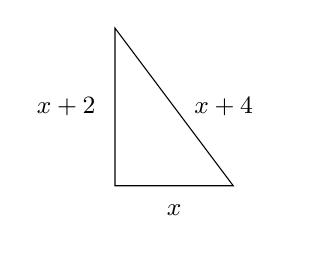
\begin{tikzpicture}[x=10mm,y=10mm,font=\small]
  \draw (1,1) -- (1,3) -- (2.5,1) -- cycle;
  \node [label={[name=label node]left:$x+2$}] at (1,2) {};
  \node [label={[name=label node]left:$x+4$}] at (3,2) {};
  \node [label={[name=label node]below:$x$}] at (1.75,1) {};
\end{tikzpicture}

\end{center}
Questa è una equazione di secondo grado in una incognita in quanto la variabile 
$x$ vi compare elevata al secondo grado.
\begin{definizione}
Si dice \emph{equazione di secondo grado}, un'equazione del tipo: $a x ^{2 } + b 
x + c = 0$ con $a, b, c \in \insR$ e $a \neq 0$. I valori $a$, $b$, $c$ prendono 
il nome di \emph{coefficienti} e, in particolare, $c$ viene detto \emph{termine 
noto}.
\end{definizione}

Un'equazione di secondo grado si definisce:
\begin{description*}
 \item \emph{monomia} quando il secondo e il terzo coefficiente sono nulli $a x 
^{2}=0$
 \item \emph{incompleta pura} quando il secondo coefficiente è nullo $a x ^{2 } 
+ c = 0$
 \item \emph{incompleta spuria} quando il terzo coefficiente è nullo $a x ^{2 } 
+ b x = 0$
 \item \emph{completa} quando i tre coefficienti sono tutti diversi da zero $a x 
^{2 } + b x + c = 0$.
\end{description*}

\subsection{Risoluzione di un'equazione di secondo grado pura}
Il coefficiente della $x$ è nullo e l'equazione si presenta nella forma: $ax ^{2 
} + c = 0$.
Si risolve portando a secondo membro il termine noto e dividendo per il 
coefficiente di $x^2$.
% \[a x ^{2 } + c = 0 \Rightarrow a x ^{2 } = - c \Rightarrow x
% ^{2 } = - \frac{c }{a } \Rightarrow x _{1,2} = \pm \sqrt{- \frac{c}{a}}.\]

Le soluzioni dell'equazione incompleta pura $ax ^{2 } + c = 0$ dipendono dal 
segno di
$- \frac{c }{a }$:
\begin{description*}
\item se $-c/a>0$, ovvero se $a$ e $c$ sono discordi, l'equazione ammette 
\emph{due soluzioni reali distinte opposte} $x _{1 } = - \sqrt{- \frac{c }{a}} 
\vee x_{2}= + \sqrt{-\frac{c}{a}}$
\item se $-c/a<0$, ovvero se $a$ e $c$ sono concordi, l'equazione \emph{non 
ammette soluzioni reali};
\item se $-c/a=0$, allora $c =0$, l'equazione ha \emph{due soluzioni reali 
coincidenti nulle} $x_{1}=x_{2} =0$.
\end{description*}

\begin{exrig}
\begin{esempio}
 Risoluzione di equazioni pure.
\begin{itemize}
\item $4 x ^{2} - 9 =0$ risoluzione
$4 x ^{2 } = + 9 \Rightarrow x ^{2 } = \frac{9 }{4 }
\Rightarrow x _{1,2 } = \pm \sqrt{\frac{9 }{4 } } \Rightarrow x_{1} = - \frac{3 
}{2 } \vee x _{2 } = + \frac{3 }{2 }$
\item $4 x ^{2 } + 9 = 0$ risoluzione $4 x ^{2 } + 9 = 0 \Rightarrow x ^{2 } = - 
\frac{9 }{4 }$. L'equazione non ammette soluzioni reali in quanto il quadrato di 
un numero reale non è mai negativo.
\end{itemize}
\end{esempio}
\end{exrig}

% \vspazio\ovalbox{\risolvii \ref{ese:3.1}, \ref{ese:3.2}, \ref{ese:3.3}, 
% \ref{ese:3.4}}

\subsection{Risoluzione di un'equazione incompleta spuria}
Un'equazione incompleta spuria si presenta nella forma: $a x ^{2 } + b x = 0$.
Per risolverla, si raccoglie a fattore comune la
$x$ precisamente $x ( a x + b ) = 0$.
Applicando la legge di annullamento del prodotto si ottiene
$x_{1} = 0$ oppure $ax + b = 0$ da cui $x_{2} = - \frac{b}{a}$.
Pertanto un'equazione di questo tipo ha sempre due soluzioni reali distinte di 
cui una nulla.
\begin{exrig}
\begin{esempio}
Risoluzione di equazioni incomplete spurie.
\begin{itemize}
\item $2 x^{2} - 4 x = 0$. Raccogliendo a fattor comune si ha: $2 x ( x - 2 ) = 
0$ da cui, applicando la legge di annullamento del prodotto, segue $2x = 0 \vee 
x - 2 = 0$ da cui $x_{1} = 0 \vee x_{2} = 2$
\item $x ^{2 } + x = 0$. Raccogliendo $x$ a fattore comune, si ha $x ( x + 1 ) = 
0$, da cui, applicando la legge di annullamento del prodotto, segue $x = 0 \vee 
x + 1 = 0$ da cui $x_{1} = 0 \vee x_{2} = - 1$.
\end{itemize}
\end{esempio}
\end{exrig}

% \vspazio
% \ovalbox{\risolvii \ref{ese:3.5}, \ref{ese:3.6}, \ref{ese:3.7}, 
%          \ref{ese:3.8}, \ref{ese:3.9}, \ref{ese:3.10}, 
%          \ref{ese:3.11}}

\section{Risoluzione di un'equazione completa}
\label{sec:eq2gr_completa}

Per risolvere l'equazione di secondo grado completa si applica una formula che 
si ottiene utilizzando il metodo del completamento del quadrato:
\begin{description*}
\item $a x^{2} + b x + c=0$: equazione completa di secondo grado;
\item $4 a^{2} x^{2} + 4 a b x + 4 a c=0$: si moltiplicano ambo i membri per 
$4a$
\item $4 a^{2} x^{2} + 4 a b x + 4 a c + b^{2}=b^{2}$: si aggiunge ad ambo i 
membri $b^{2}$
\item $4 a^{2} x^{2} + 4 a b x + b^{2}=b^{2} - 4 a c$: si porta $4ac$ a secondo 
membro;
\item $( 2 a x + b )^{2}=b^{2} - 4 a c$: il primo membro risulta il quadrato di 
un binomio;
\item $k=2 a x + b$: si sostituisce il binomio $2ax + b$ con la la variabile $k$
\item $k^{2}=b^{2} - 4 a c$: l'equazione diventa un'equazione di secondo grado 
pura in $k$
\item $k_{1,2}=\pm \sqrt{b^{2} - 4 a c}$: si calcolano le soluzioni in $k$
 (attenzione però al segno del radicando!)
\item $2 a x + b=\pm \sqrt{b^{2} - 4 a c}$: al posto di $k$ si mette il binomio 
$2ax + b$
\item $2 a x=- b \pm \sqrt{b^{2} - 4 a c}$: si separa il monomio con 
l'incognita;
\item $x_{1,2}=\frac{- b \pm \sqrt{b^{2} - 4 a c}}{2 a}$: si risolve l'equazione 
di primo grado rispetto alla $x$.
\end{description*}

Da quanto ottenuto possiamo osservare che:
\begin{itemize}
\item la soluzione si ottiene esclusivamente operando sui coefficienti
dell'equazione;
\item il valore dell'incognita si ottiene con due calcoli: $x_{1} = \frac{- b - 
\sqrt{b^{2} - 4 ac}}{2 a}$ e $ x_{2} = \frac{- b + \sqrt{b^{2} - 4 ac}}{2 a}$
\item nel calcolo è coinvolta l'estrazione di radice quadrata: l'espressione 
$b^{2} - 4 ac$ prende il nome di \emph{discriminante} e si è solito porre
$b^{2} - 4 ac = \Delta (\text{ Delta})$.
\end{itemize}

Questa formula si può applicare anche ai tipi di equazioni incomplete che 
abbiamo già studiato. La parola discriminante deriva dal verbo \emph{discrimen} 
(divisione); in effetti, il $\Delta$ permette di effettuare una distinzione tra 
la tipologia delle soluzioni di un'equazione di secondo grado.
Si possono infatti presentare tre casi:
\begin{itemize}
\item Primo caso. $\Delta=b^{2} - 4 a c > 0$ il radicale $\sqrt{\Delta}$ è un 
numero reale e l'equazione ammette \emph{due soluzioni reali e
distinte}: $x_{1}=\frac{- b - \sqrt{\Delta}}{2 a} \vee x_{2} = \frac{- b + 
\sqrt{\Delta}}{2 a}$
\item Secondo caso. $\Delta=b^{2} - 4 a c=0$ l'equazione ammette \emph{due 
radici reali e coincidenti}: $x_{1}=x_{2}=- \frac{b}{2 a}$
\item Terzo caso. $\Delta=b^{2} - 4 a c < 0$, l 'equazione \emph{non ammette 
soluzioni reali}.
\end{itemize}

Riassumendo e schematizzando si ha:
\begin{center}
\begin{tabular}{ll}
\toprule
\multicolumn{2}{c} {$a x^{2} + b x + c=0$ con~$a \neq 0$}\vspace{1.05ex}\\
Discriminante & Soluzioni\\
\midrule
$\Delta > 0$ & Due soluzioni reali e distinte: $x_{1}=\frac{- b - 
\sqrt{\Delta}}{2 a} \vee x_{2} = \frac{- b + \sqrt{\Delta}}{2 a}$\\
$\Delta = 0$ & Due soluzioni reali e coincidenti: $x_{1}=x_{2}=- \frac{b}{2 a}$ 
\\
$\Delta < 0$ & Nessuna soluzione reale: $I.S.=\emptyset$ \\
\bottomrule
\end{tabular}
\end{center}

\begin{exrig}
\begin{esempio}
Risoluzione di equazioni complete.
\begin{itemize}
\item $3 x^{2} - 5 x + 2=0$. $a = + 3, b = - 5, c = + 2$. Calcolo del 
discriminante: 
\[\Delta = b^{2} - 4 ac = ( - 5 )^{2} - 4 ( + 3 ) ( + 2 ) = 25 - 24 = 1.\]
 Poiché $\Delta > 0$ l'equazione ammette due soluzioni reali e distinte 
\[x_{1,2} = \frac{- b \pm \sqrt{\Delta}}{2 a} \Rightarrow x_{1,2} = \frac{- (- 
5) \pm \sqrt{1}}{( + 2 ) ( + 3 )} \Rightarrow x_{1,2} = \frac{5 \pm 1}{6} 
\Rightarrow x_{1} = 1 \vee x_{2} = \frac{2}{3};\]
\item $4 x^{2} - 12 x + 9=0$. $a = + 4, b = - 12, c = + 9$. Calcolo del 
discriminante: 
\[\Delta=( - 12 )^{2} - 4 ( + 4 ) ( + 9 )=144 - 144 =0.\] 
Poiché $\Delta = 0$ l'equazione ammette due soluzioni reali coincidenti 
\[x_{1,2} = - \frac{b}{2 a} \Rightarrow x_{1,2} = \frac{- ( - 12)}{2 ( + 4 )} = 
\frac{12}{8} \Rightarrow x_{1} = x_{2} = \frac{3}{2};\]
\item $x^{2} - x + 3=0$. $a = + 1, b = - 1, c = + 3$. Calcolo del 
discriminante: 
\[\Delta = ( - 1 )^{2} - 4 ( + 1 ) ( + 3 ) = 1 - 12 = - 11.\] Poiché $\Delta < 
0$ l'equazione non ammette soluzioni reali.
\end{itemize}
\end{esempio}
\end{exrig}

% \vspazio
% \ovalbox{\risolvii \ref{ese:3.12}, \ref{ese:3.13}, \ref{ese:3.14}, 
%                    \ref{ese:3.15}, \ref{ese:3.16}, \ref{ese:3.17}, 
%                    \ref{ese:3.18}, \ref{ese:3.19}}
% \vspazio

\subsection{Formula ridotta per equazioni di secondo grado}
Se nell'equazione
$a x^{2} + b x + c=0$ il coefficiente $b$ è un numero pari, conviene applicare 
una formula, detta \emph{formula ridotta}, che semplifica i calcoli.

Supponiamo $b=2 k$, l'equazione $a x^{2} + b x + c=0$ diventa $a x^{2} + 2 k x + 
c=0$ e nella formula risolutiva dell'equazione si ottiene:
\[x_{1,2}=\frac{- 2 k \pm \sqrt{( 2 k )^{2}-4 a c}}{2 a}=\frac{- 2 k \pm 2 
\sqrt{k^{2} - a c}}{2 a}=\frac{- k \pm \sqrt{k^{2} - a c}}{a}.\]
Dato che $b=2 k$ quindi $k=\frac{b}{2}$ la formula ridotta che conviene 
utilizzare quando $b$ è pari è:
\[x_{1,2}=\frac{\left( - \frac{b}{2} \right) \pm \sqrt{\left(\frac{b}{2} 
\right)^{2} - a c}}{a}.\]

La quantità sotto radice, uguale a $\frac{\Delta}{4}$, è detta anche 
\emph{discriminante ridotto}.

\begin{exrig}
\begin{esempio}
 Applicazione della formula ridotta nella risoluzione di equazioni complete.
\begin{itemize}
\item $x^{2} - 4 x + 3=0$. Il coefficiente di primo grado è pari, per cui 
conviene utilizzare la formula ridotta: 
\[\frac{-(-2 ) \pm \sqrt{(-2)^{2}-1( 3 )}}{1}=2 \pm \sqrt{1}\Rightarrow  x_{1} = 
1 \vee x_{2} = 3;\]
\item $- x^{2} - 2 x + 24=0$. Applichiamo la formula ridotta: 
\[\frac{- ( - 1 ) \pm \sqrt{( -1 )^{2} - ( - 1 ) ( 24 )}}{- 1}=- 1 \pm 
\sqrt{25}\Rightarrow x_{1} = - 6 \vee x_{2} = 4;\]
\item $- 3 x^{2} - 6 x + 12=0$. Per prima cosa dividiamo l'equazione per $- 3$, 
per il secondo principio di equivalenza, si ha l'equazione equivalente~$x^{2} + 
2 x - 4=0$. Poiché il coefficiente della~$x$ è pari si può applicare la formula 
ridotta: 
\[x_{1,2}=- 1 \pm \sqrt{1 + 4} = - 1\pm \sqrt{5}\Rightarrow x_{1} = - 1 + 
\sqrt{5} \vee x_{2} = - 1 - \sqrt{5}.\]
\end{itemize}
\end{esempio}
\end{exrig}

Quando $b$ è pari e $a = 1$, la formula si dice \emph{ridottissima}: 
$x_{1,2}=\left( - \frac{b}{2} \right) \pm \sqrt{\left( \frac{b}{2} \right)^{2} - 
c}$.

\begin{exrig}
\begin{esempio}
 Applicazione della formula ridottissima nella risoluzione di equazioni 
complete.
\begin{itemize}
\item $x^{2} - 6 x + 8 = 0$. Il coefficiente $b$ è pari e il coefficiente $a=1$, 
quindi possiamo applicare la formula ridottissima $x_{1,2} = 3 \pm \sqrt{9 - 
8}$, quindi $x_{1}=2 \vee x_{2} = 4$.
\end{itemize}
\end{esempio}
\end{exrig}
% \vspazio
% \ovalbox{\risolvii \ref{ese:3.20}, \ref{ese:3.21}, 
%                    \ref{ese:3.22}, \ref{ese:3.23}, 
%                    \ref{ese:3.24}}
% \vspazio

Riassumiamo e schematizziamo la risoluzione di un'equazione di secondo grado:
\begin{center}
\begin{tabular}{llll}
\toprule
\multicolumn{4}{c} {Equazioni incomplete}\vspace{1.05ex}\\
Coefficienti & Nome & Equazione & Soluzioni\\
\midrule
$b = 0, c = 0$ & Monomia & $a x^{2}=0$ & $x_{1}=x_{2}=0$\\
$b = 0, c \neq 0$ & Pura & $a x^{2} + c=0$ & $\IS=\emptyset$ se~$a \cdot c>0$\\
& & & $x_{1,2} = \pm \sqrt{- \frac{c}{a}}$ se~$a \cdot c<0$\\
$b \neq 0, c = 0$ & Spuria & $a x^{2} + b x=0$ & $x_{1} = 0 \vee x_{2} = - 
\frac{b}{a}$ \vspace{1.1ex}\\
\toprule
\multicolumn{4}{c} {Equazione completa \, $ax^2+bx+c=0$}\vspace{1.05ex}\\
Discriminante & \multicolumn{2}{l} {Numero soluzioni} & Soluzioni\\
\midrule
$\Delta > 0$ & \multicolumn{2}{l} {Due soluzioni reali e distinte}& 
$x_{1,2}=\frac{-b\pm{\sqrt {b^{2}-4ac}}}{2a}$\\
$\Delta = 0$ & \multicolumn{2}{l} {Due soluzioni reali e coincidenti} & 
$x_{1}=x_{2}=-\frac{b}{2a}$\\
$\Delta < 0$ & \multicolumn{2}{l} {Nessuna soluzione reale}& $\IS=\emptyset$\\
\bottomrule
\end{tabular}
\end{center}

% \vspazio
% \ovalbox{\risolvii \ref{ese:3.25}, \ref{ese:3.26}, \ref{ese:3.27}, 
%          \ref{ese:3.28}, \ref{ese:3.29}, \ref{ese:3.30}, \ref{ese:3.31}, 
%          \ref{ese:3.32}, \ref{ese:3.33}, \ref{ese:3.34}, \ref{ese:3.35}}
% \vspazio

% \subsection{Equazioni che si possono risolvere con opportune sostituzioni}
% 
% \begin{exrig}
% \begin{esempio}
% Risoluzione di equazioni con sostituzioni.
% \begin{itemize}
% \item $( x - 1 )^{2} = 16$. Sostituendo $x - 1 = t$ l'equazione diventa $t^{2} = 
% 16$, le cui soluzioni sono $t_{1} = - 4 \vee t_{2} = + 4$. Per determinare la 
% $x$ sostituiamo i valori di $t$ trovati nella relazione~$x - 1 = t$. Si ha $x - 
% 1 = - 4 \vee x - 1 = + 4$ quindi l'equazione assegnata ammette le due soluzioni
% $x_{1} = - 3 \vee x_{2} = 5$
% \item $( x - 1 )^{2} + 2 ( x - 1 ) = 0$. Sostituendo $x - 1 = t$ l'equazione 
% diventa $t^{2} + 2t = 0$ le cui soluzioni sono $t ( t + 2 ) = 0 \Rightarrow 
% t_{1} = 0 \vee t + 2 = 0 \Rightarrow t_{2} = - 2$. Sostituendo $x - 1 = t$ si ha 
% $x - 1 = 0 \vee x - 1 = - 2$ quindi l'equazione assegnata ammette le due 
% soluzioni~$x_{1} = - 1 \vee x_{2} = 1$.
% \end{itemize}
% \end{esempio}
% \end{exrig}
% \vspazio\ovalbox{\risolvii \ref{ese:3.36}, \ref{ese:3.37}, \ref{ese:3.38}}

\section{Equazioni numeriche frazionarie}
\label{sec:eq2gr_frazionarie}

Un'equazione in cui compare l'incognita al denominatore si chiama 
\emph{frazionaria o fratta.}

\begin{exrig}
\begin{esempio}
Risolvere la seguente equazione $\dfrac{3 x + 2}{1 + x}=\dfrac{2 x + 3}{x - 2}$.
 \paragraph{Passo I} Determiniamo il $\mcm$ dei denominatori: $\mcm = ( 1 + x ) 
\cdot ( x - 2 )$.
 \paragraph{Passo II} Imponiamo le \emph{Condizioni} di \emph{Esistenza} 
($\CE$): $\CE x \neq - 1 \wedge x \neq 2$. La ricerca dei valori che risolvono 
l'equazione si restringe ai numeri reali appartenenti all'insieme, $\Dom = \insR 
- \{- 1, 2 \}$ detto \emph{Dominio} dell'equazione o \emph{Insieme} di 
\emph{Definizione} (abbreviato $\ID$).
 \paragraph{Passo III} Applichiamo il primo principio d'equivalenza trasportando 
al primo membro la frazione del secondo membro $\frac{3 x + 2}{1 + x} - \frac{2 
x + 3}{x - 2} = 0$. Riduciamo allo stesso denominatore ($\mcm$): 
\[\frac{( 3 x + 2 ) \cdot ( x - 2 ) - ( 2 x + 3 ) \cdot ( 1 + x )}{( 1 +x ) 
\cdot ( x - 2 )}=0.\]
 \paragraph{Passo IV} Moltiplichiamo ambo i membri per il $\mcm$, certamente 
diverso da zero per le condizioni poste; l'equazione diventa: $( 3 x + 2 ) \cdot 
( x - 2 ) - ( 2 x + 3 ) \cdot ( 1 + x )=0$.
 \paragraph{Passo V} L'equazione che si ottiene è di secondo grado; portiamo 
l'equazione alla forma canonica: $3 x^{2} - 6 x + 2 x - 4 - 2 x - 3 - 2 x^{2} - 
3 x=0 \Rightarrow x^{2} - 9 x - 7=0$.
 \paragraph{Passo VI} Calcoliamo il discriminante: $\Delta=b^{2} - 4 a c=81 + 28 
= 109$. Il discriminante è positivo quindi l'equazione è determinata e ammette 
due soluzioni reali distinte: 
\[x_{1,2}=\frac{9 \pm \sqrt{109}}{2} \Rightarrow x_{1}=\frac{9 - \sqrt{109}}{2} 
\vee x_{2}=\frac{9 + \sqrt{109}}{2}.\]
 \paragraph{Passo VII} Confrontiamo le soluzioni con le Condizioni di Esistenza; 
in questo caso le radici appartengono all'insieme \emph{D}; diciamo che sono 
accettabili e l'insieme soluzione è: $\IS=\left\{\frac{9 - \sqrt{109}}{2}, 
\frac{9 +\sqrt{109}}{2} \right\}$.
 \end{esempio}

 \begin{esempio}
Risolvere la seguente equazione $\dfrac{x^{2}}{x^{2} - 3 x + 2}=\dfrac{x - 2}{x 
- 1} +\dfrac{1}{x + 2}$.
 \paragraph{Passo I} Determiniamo il $\mcm$ dei denominatori. Scomponiamo in 
fattori i denominatori. Riscriviamo: $\frac{x^{2}}{( x - 2 ) ( x - 1 )}=\frac{x 
- 2}{x - 1} +\frac{1}{x + 2}$ il $\mcm$ è $( x - 2 ) ( x - 1 ) ( x + 2 )$.
 \paragraph{Passo II} Imponiamo le Condizioni di Esistenza: $\CE x \neq 1 \wedge 
x \neq 2 \wedge x \neq - 2$ quindi $\Dom = \insR - \{ 1, 2, - 2 \}=\ID$
 \paragraph{Passo III} Trasportiamo al primo membro ed uguagliamo a zero; 
riduciamo allo stesso denominatore ($\mcm$) i membri dell'equazione: 
\[\frac{x^{3} + 2 x^{2} - x^{2} + 3 x - 2 - x^{3} - 2 x^{2} + 4x^{2} + 8 x - 4 x 
- 8}{( x - 2 ) ( x - 1 ) ( x + 2 )}~=~0.\]
 \paragraph{Passo IV} Applichiamo il secondo principio di equivalenza 
moltiplicando ambo i membri per il $\mcm$, certamente diverso da zero per le 
condizioni poste in precedenza; l'equazione diventa: $3 x^{2} + 7 x - 10 = 0$.
 \paragraph{Passo V} Calcoliamo il discriminante: $\Delta=b^{2} - 4 a c=49 + 
120=169$. Il discriminante è positivo, l'equazione determinata e ammette due 
soluzioni reali distinte: $x_{1,2}=\frac{- 7 \pm 13}{6}$ 
cioè~$x_{1}=-\frac{10}{3} \vee x_{2}=1$.
 \paragraph{Passo VI} Confrontiamo con le $\CE$ in questo caso solo $x_{1}$ 
appartiene all'insieme $\Dom$ diciamo che l'insieme soluzione è: 
$\IS=\left\{-\frac{10}{3}\right\}$ mentre $x_{2} = 1$ non è accettabile.
\end{esempio}
\end{exrig}
% \vspazio\ovalbox{\risolvii \ref{ese:3.39}, \ref{ese:3.40}, \ref{ese:3.41}, 
% \ref{ese:3.42}, \ref{ese:3.43}, \ref{ese:3.44}, \ref{ese:3.45}, \ref{ese:3.46}, 
% \ref{ese:3.47}, \ref{ese:3.48}, \ref{ese:3.49}, \ref{ese:3.50}, \ref{ese:3.51},}
% 
% \vspazio\ovalbox{\ref{ese:3.52}, \ref{ese:3.53}}

% \section{Discussione e risoluzione di equazioni letterali}
% \label{sec:eq2gr_letterali}
% 
% Ricordiamo la seguente definizione:
% \begin{definizione}
% Una equazione è \emph{letterale} se i coefficienti dell'incognita sono 
% espressioni letterali, cioè se oltre all'incognita (in genere indicata con
% la lettera $x$) compare un'altra lettera (in genere $a, b, k, \ldots$) detta 
% parametro.
% \end{definizione}
% 
% \begin{exrig}
% \begin{esempio}
% Data l'equazione $k x^{2} - ( 2 k - 1 ) x + ( k - 3 ) = 0$, discutere al variare 
% di $k$ la realtà delle sue soluzioni.
% 
% L'equazione è letterale di secondo grado nell'incognita $x$, i cui coefficienti 
% dipendono dal parametro $k$. Il parametro $k$ può assumere qualunque valore 
% numerico e l'equazione rappresenta una famiglia di equazioni le cui 
% caratteristiche variano a seconda dei valori attribuiti al parametro. Notiamo 
% subito che se
% $k$ assume il valore zero, l'equazione non è più di secondo grado. Se $k$ assume 
% il valore $3$, l'equazione è ancora di secondo grado ma è incompleta (spuria) 
% perché priva del termine noto.
% 
% \emph{Discutere} un'equazione letterale di secondo grado significa analizzare 
% come varia il suo insieme delle soluzioni al variare del parametro.
% 
% Ricordando la formula $x_{1,2}=\frac{- b \pm \sqrt{b^{2} - 4 a c}}{2 a}$ in cui 
% compaiono i tre coefficienti $a, b, c$ possiamo dire che:
%  \begin{itemize*}
%  \item il primo coefficiente è $k$, se $k = 0$ l'equazione diventa $x - 3 = 0$ 
% di primo grado con $\IS = \{3\}$
%  \item il secondo coefficiente è $-2k+1$, se questo è nullo, ossia se $k = 
% \frac{1}{2}$ l'equazione diventa $\frac{1}{2} x^{2} - \frac{5}{2}=0$, equazione 
% pura con due soluzioni reali opposte $x_{1} = - \sqrt{5} \vee x_{2} = \sqrt{5}$
%  \item il terzo coefficiente è $k-3$, se è nullo, cioè se $k = 3$ l'equazione 
% diventa $3 x^{2} - 5 x = 0$, equazione spuria con due soluzioni reali $x_{1} = 0 
% \vee x_{2} = \frac{5}{3}$.
%  \end{itemize*}
% 
% Per tutti i valori di $k$ dell'insieme $\insR - \left\{ 0, \frac{1}{2},3 
% \right\}$ l'equazione è completa, l'esistenza di soluzioni reali dipende dal 
% discriminante $\Delta = \left( - 2 k + 1 \right)^{2} - 4 k \left( k - 3 \right) 
% = 8 k + 1$, quindi se
% \begin{itemize*}
%  \item $8 k + 1 < 0 \Rightarrow k < - \frac{1}{8}$ l'equazione non ammette 
% soluzioni reali e $\IS = \emptyset$
%  \item $8 k + 1 \geq 0 \Rightarrow k \geq - \frac{1}{8}$. In particolare se $ 
% k>-\frac{1}{8} $ l'equazione ammette due soluzioni reali distinte $ x_{1,2} = 
% \frac{\left(2 k - 1 \right) \pm \sqrt{8 k + 1}}{2 k}$, se $ k=- \frac{1}{8} $ 
% coincidenti $ x_{1} = x_{2}=5$.
% \end{itemize*}
% Riassumendo e schematizzando si ha:
% \begin{center}
% \begin{tabular}{lll}
% \toprule
% \multicolumn{3}{c} {$k x^{2} - ( 2 k - 1 ) x + ( k - 3 ) = 0$ con $k \in 
% \insR$}\vspace{1.05ex}\\
% Parametro & Insieme Soluzione & Equazione\\
% \midrule
% $k = 0$ & $x = 3$ & di primo grado\\
% $k = \frac{1}{2}$ & $x_{1} = - \sqrt{5} \vee x_{2} = + \sqrt{5}$ & pura\\
% $k = 3$ & $x_{1} = 0 \vee x_{2} = \frac{5}{3}$ & spuria\\
% $k \in \insR - \left\{ 0, \frac{1}{2}, 3 \right\}$ & & completa, $\Delta = 8 k + 
% 1$\\
% $k < - \frac{1}{8}$ & $\Delta < 0$ non esistono soluzioni reali $I.S. = 
% \emptyset$& \\
% $k \geq - \frac{1}{8}$ & $\Delta \geq 0$ esistono soluzioni reali & \\
% $k > - \frac{1}{8}$ & $x_{1}=\frac{\left( 2 k - 1 \right) - \sqrt{8 k + 
% 1}}{2k}\vee x_{2}=\frac{\left( 2 k - 1 \right) + \sqrt{8 k + 1}}{2 k}$ & \\
% $k = - \frac{1}{8}$ & $x_{1} = x_{2}=5$ &\\
% \bottomrule
% \end{tabular}
% \end{center}
% \end{esempio}
% 
% \begin{esempio}
% Data l'equazione $x^2 - 3 x + 1 - k = 0$, discutere al variare di $k \in \insR$, 
% la realtà delle radici.
% 
% Il primo e il secondo coefficiente non dipendono dal parametro $k$, quindi 
% analizziamo il terzo coefficiente. Se $k = 1$ l'equazione diventa un'equazione 
% spuria con due radici reali $x_{1} = 0 \vee x_{2} = 3$. Per tutti i valori di 
% $k$ dell'insieme $\insR - \{1\}$ l'equazione è completa, l'esistenza di 
% soluzioni reali dipende dal discriminante $\Delta = 9 - 4 ( 1 - k ) = 4 k + 5$, 
% quindi se:
% \begin{itemize*}
%  \item $k < - \frac{5}{4}$ l'equazione non ammette soluzioni reali e $\IS = 
% \emptyset$
%  \item $k \geq - \frac{5}{4}$ l'equazione ammette due radici reali distinte se 
% $k >-\frac{5}{4}\Rightarrow x_{1,2} =\frac{3 \pm\sqrt{4 k +5}}{2}$, coincidenti 
% se $k=- \frac{5}{4} \Rightarrow x_{1} = x_{2} = \frac{3}{2}$.
% \end{itemize*}
% Riassumendo e schematizzando si ha:
% \begin{center}
% \begin{tabular}{lll}
% \toprule
% \multicolumn{3}{c} {$x^{2} - 3 x + 1 - k = 0$ con $k \in 
% \insR$}\vspace{1.05ex}\\
% Parametro & Insieme Soluzione & Equazione\\
% \midrule
% $k = 1$ & $x_{1} = 0 \vee x_{2} = 3$ & spuria\\
% $k \in \insR - \{1\}$ & & completa, $\Delta = 4 k + 5$\\
% $k < - \frac{5}{4}$ & $\Delta < 0$ non esistono soluzioni reali $I.S. = 
% \emptyset$& \\
% $k \geq - \frac{5}{4}$ & $\Delta \geq 0$ esistono soluzioni reali & \\
% $k > - \frac{5}{4}$ & $x_{1}=\frac{3 - \sqrt{4 k + 5}}{2} \vee x_{2}=\frac{3 + 
% \sqrt{4 k + 5}}{2}$ & \\
% $k = - \frac{5}{4}$ & $x_{1} = x_{2}=\frac{3}{2}$ &\\
% \bottomrule
% \end{tabular}
% \end{center}
% \end{esempio}
% 
% \begin{esempio}
% Discutere la seguente equazione letterale: $\frac{x^{2}}{m - 1} + 3 + m=\frac{2 
% m x}{m - 1} \left( 1 +\frac{1}{m} \right)$.
% 
% L'equazione pur presentando delle frazioni è intera, in quanto l'incognita $x$ 
% non compare al denominatore. Se~$m = 0$ oppure~$m = 1$ l'equazione è priva di 
% significato, quindi le Condizioni di Esistenza sono $ m \neq 0 \wedge m \neq 1$.
% 
% Trasportiamo a sinistra del segno di uguaglianza i termini di destra ed 
% eseguiamo il calcolo nella parentesi: 
% \[\frac{x^{2}}{m - 1} + 3 + m - \frac{2 m x}{m - 1} \left( 1 +\frac{1}{m} 
% \right) = 0 \Rightarrow \frac{x^{2}}{m - 1} + 3 + m - \frac{2 m x}{m - 1} - 
% \frac{2 m x}{m - 1} \cdot \frac{1}{m} = 0.\]
% Semplifichiamo $m$ nell'ultimo termine, poiché nelle $\CE m \neq 0$, si ottiene
% \[\frac{x^{2}}{m - 1} + 3 + m - \frac{2 mx}{m - 1} - \frac{2 x}{m - 1}=0.\]
% Riduciamo allo stesso denominatore $m - 1$, eliminiamo il denominatore essendo 
% $m \neq 1$ per le $\CE$ si ha: $x^{2} + 3 m - 3 + m^{2} - m - 2 m x - 2 x = 0$.
% Scriviamo l'equazione di secondo grado in forma canonica $x^{2} - 2 x ( m + 1 ) 
% + m^{2} + 2 m - 3 = 0$.
% 
% \emph{Discussione}
% \begin{itemize*}
% \item il primo coefficiente essendo uguale a $1$ non dipende dal valore del 
% parametro, quindi l'equazione è di secondo grado per qualunque valore di $m \in 
% \insR - \{0, 1\}$
% \item il secondo coefficiente è $- 2 (m + 1)$: se $m = - 1$ l'equazione diventa 
% $x^{2} - 4 = 0$, equazione pura con due soluzioni reali opposte $x_{1} = - 2 
% \vee x_{2} = 2$
% \item il terzo coefficiente è $m^{2} + 2 m - 3$: se $m^{2} + 2 m - 3 = 0 
% \Rightarrow m = 1 \vee m = - 3$ (non consideriamo il caso $m = 1$ per le $\CE$) 
% l'equazione diventa $x^{2} + 4 x = 0$, equazione spuria con due soluzioni reali 
% $x_{1} = 0 \vee x_{2} = - 4$.
% \end{itemize*}
% Prima conclusione: per tutti i valori di $m$ nell'insieme $\insR -\{ 0, 1, -1, 
% -3 \}$ l'equazione è completa e l'esistenza di soluzioni reali dipende dal 
% discriminante. Calcoliamo il discriminante: $\frac{\Delta}{4}~=~( m + 1 )^{2} - 
% ( m^{2} + 2 m - 3 ) = 4$ esso risulta indipendente dal valore del parametro~$m$ 
% e sempre positivo, l'equazione ammette due soluzioni reali distinte $x_{1} = m - 
% 1 \vee x_{2} = m + 3$.
% 
% Riassumendo in una tabella tutti i risultati ottenuti:
% \begin{center}
% \begin{tabular}{lll}
% \toprule
% \multicolumn{3}{c} {$\frac{x^{2}}{m - 1} + 3 + m=\frac{2 m x}{m - 1} \left( 1 + 
% \frac{1}{m} \right)$ con $m \in \insR$}\vspace{1.05ex}\\
% Parametro & Insieme Soluzione & Equazione\\
% \midrule
% $m = 0 \vee m=1$ & & priva di significato\\
% $m =-1$ & $x_{1}=- 2 \vee x_{2}=2$ & pura\\
% $m = - 3$ & $x_{1}=0 \vee x_{2}=- 4$ & spuria\\
% $m \in \insR - \{ 0, 1,-1, -3 \}$ & $x_{1} = m - 1 \vee x_{2} = m + 3$ & 
% completa: $\Delta = 4$\\
% \bottomrule
% \end{tabular}
% \end{center}
% \end{esempio}
% % 8<
% \begin{esempio}
% Discutere l'equazione parametrica $\frac{k + x}{2 x} \left( \frac{k + x}{k - x} 
% + \frac{k - x}{k + x} \right)=k + \frac{2 k}{k x - x^{2}} - 1$.
% 
% L'equazione è fratta, poiché nel denominatore compare l'incognita $x$. 
% Trasportiamo i termini del secondo membro a sinistra del segno uguale e 
% scomponiamo in fattori i denominatori: 
% \[\frac{k + x}{2 x} \left( \frac{k + x}{k - x} + \frac{k - x}{k +x} \right) - k 
% - \frac{2 k}{x ( k - x )} + 1=0; \CE x \neq 0 \wedge x \neq k \wedge x \neq - 
% k.\]
% Svolgiamo i calcoli nella parentesi e moltiplichiamo $\frac{k^{2} + x^{2}}{x ( k 
% - x )} - k - \frac{2 k}{x ( k - x )} + 1=0$
% Riduciamo allo stesso denominatore ed eliminiamo il denominatore $k x^{2} + k x 
% \cdot ( 1 - k ) + k \cdot ( k - 2 )=0$
% 
% \emph{Discussione}
% \begin{itemize}
%  \item Il primo coefficiente è $k$, se $k = 0$ le $\CE$ si riducono a $x \neq 0$ 
% e l'equazione diventa $0x = 0$ indeterminata, quindi $I.S. = \insR - \{ 0\}$ per 
% le condizioni poste sull'incognita. Avendo studiato il caso $k=0$, possiamo ora 
% supporre $k \neq 0$, dividiamo tutti i coefficienti per $k$, l'equazione diventa 
% $x^{2} + x \cdot ( 1 - k ) + ( k - 2 )=0$
%  \item il secondo coefficiente è $1-k$, se $k = 1$ le $\CE$ sono $x \neq 0 
% \wedge x \neq 1 \wedge x \neq - 1$ e l'equazione diventa $x^{2} - 1 = 0$, le 
% soluzioni sono $x_{1} = -1 \vee x_{2} = 1$ che non sono accettabili per le $\CE$
%  \item il terzo coefficiente è $k-2$, se $k = 2$ le $\CE$ sono $x \neq 0 \wedge 
% x \neq 2 \wedge x \neq - 2$ e l'equazione diventa $x^{2} - x = 0$ le cui 
% soluzioni sono $x_{1} = 0 \vee x_{2} = 1$ di cui $x_{1} = 0$ non accettabile per 
% le $\CE$
% \end{itemize}
% Per $k \in \insR - \{0, 1, 2\}$ l'equazione è completa, l'esistenza di soluzioni 
% reali dipende dal discriminante $\Delta = (1 - k)^{2}-4(k-2)=(k-3)^{2}$, essendo
% $\Delta \geq 0\, \forall k$, si avranno sempre due soluzioni reali: coincidenti 
% se $k = 3 \Rightarrow x_{1} = x_{2} = 1$ accettabili essendo le
% $\CE x \neq - 3 \wedge x \neq 0 \wedge x \neq 3$ distinte se $k \neq 3 
% \Rightarrow x_{1} = 1 \vee x_{2} = k - 2$ e confrontando con le C.E. si ottiene 
% $x_{1} = 1$
% non accettabile se $k = - 1$ $x_{2}$ sempre accettabile per $k \in \mathbb{R} - 
% \{ 0,1,2,3, - 1 \}$.
% % >8
% Riassumendo in una tabella tutti i risultati ottenuti:
% \begin{center}
% \begin{threeparttable}
% \begin{tabular}{llll}
% \toprule
% \multicolumn{3}{c} {$\frac{k + x}{2 x} \left( \frac{k + x}{k - x} + \frac{k - 
% x}{k + x} \right)=k + \frac{2 k}{k x - x^{2}} - 1$ con $m \in 
% \insR$}\vspace{1.05ex}\\
% Parametro & Incognita & Insieme Soluzione & Equazione\\
% \midrule
%  & $x \neq -k \wedge x \neq 0 \wedge x \neq k$ & & \\
% $k = 0$ & $x \neq 0$ & $\IS= \insR - \{ 0\}$ & indeterm.\\
% $k = 1$ & $x \neq -1 \wedge x \neq 0 \wedge x \neq 1$ & $[x_{1} = - 1 \vee x_{2} 
% = 1]^{*}$ & pura\\
% $k = 2$ & $x \neq -2 \wedge x \neq 0 \wedge x \neq 2$ & $x_{1} = 0^{*} \vee 
% x_{2} = 1$ & spuria\\
% $k \in \insR - \{0, 1, 2 \}$ & & & completa\\
% $k = 3$ & $x \neq - 3 \wedge x \neq 0 \wedge x \neq 3$ & $x_{1} = x_{2} = 1$ & 
% \\
% $k \in \insR - \{0, 1, 2, 3 \}$ & $x \neq - k \wedge x \neq 0 \wedge x \neq k$ & 
% $x_{1} = 1 \vee x_{2} = k - 2$ & \\
% $k = - 1$ & & $x_{1} = 1^{*}$ & \\
% $k \in \insR -\{0, 1, 2, 3, -1 \}$ & & $x_{2} = k - 2$ & \\
% \bottomrule
% \end{tabular}
% \begin{tablenotes}
% \item [*] La soluzione o le soluzioni non sono accettabili.
% \end{tablenotes}
% \end{threeparttable}
% \end{center}
% \end{esempio}
% % >8
% \end{exrig}
% \vspazio\ovalbox{\risolvii \ref{ese:3.54}, \ref{ese:3.55}, \ref{ese:3.56}, 
% \ref{ese:3.57}, \ref{ese:3.58}, \ref{ese:3.59}, \ref{ese:3.60}, \ref{ese:3.61}, 
% \ref{ese:3.62}, \ref{ese:3.63}, \ref{ese:3.64}, \ref{ese:3.65}, \ref{ese:3.66}.}

\section{Relazioni tra soluzioni e coefficienti}
\label{sec:eq2gr_coefficienti}

Consideriamo una generica equazione di secondo grado $a x^{2} + b x + c = 0$ 
nell'ipotesi in cui ammetta soluzioni reali (cioè $\Delta \geq 0$), sommiamo e 
moltiplichiamo le soluzioni (o radici) dell'equazione:
\begin{align*}
& x_{1} + x_{2} = \frac{- b - \sqrt{\Delta}}{2 a} + \frac{- b + \sqrt{\Delta}}{2 
a} = - \frac{2 b}{2 a}=- \frac{b}{a};\\
& x_{1} \cdot x_{2}=\left( \frac{- b - \sqrt{\Delta}}{2 a} \right) \cdot \left( 
\frac{- b + \sqrt{\Delta}}{2 a} \right)= \frac{b^{2} - \Delta}{4 
a^2}=\frac{b^{2} + 4 a c - b^{2}}{4 a^{2}} =\frac{4 a c}{4 a^{2}}=\frac{c}{a}.
\end{align*}
Quindi, la somma delle radici è $x_{1} + x_{2}=- \dfrac{b}{a}$ e il prodotto 
delle radici è $x_{1} \cdot x_{2}=\dfrac{c}{a}$.

Osserviamo che queste relazioni tra radici e coefficienti dell'equazione valgono 
anche nel caso in cui le radici non siano reali ($\Delta<0$).
\begin{exrig}
\begin{esempio}
Determinare somma e prodotto delle soluzioni dell'equazione $a x^{2} + b x +c = 
0$ senza risolverla.
 \begin{itemize}
 \item $2 x^{2} + 11 x - 3 = 0$.

 Calcolo il discriminante $\Delta = 145 > 0$ pertanto le radici sono reali e 
distinte. Applicando le precedenti formule si ha: 
\[x_{1} + x_{2} = - \frac{11}{2}; x_{1} \cdot x_{2} = - \frac{3}{2}.\]

 \item $x^{2} \sqrt{2} + 3 x - 2 \sqrt{2} = 0$.
 Calcolo il discriminante $\Delta = 25 > 0$ pertanto le radici sono reali e 
distinte. Applicando le precedenti formule si ha: 
\[x_{1} + x_{2} = - \frac{3}{\sqrt{2}} = - \frac{3 \sqrt{2}}{2}; x_{1} \cdot 
x_{2} = - \frac{2 \sqrt{2}}{\sqrt{2}} = - 2.\]

 \item $x^{2} + 2 x + 15 = 0$.

 Calcolo il discriminante $\Delta = - 56 < 0$ le radici non sono reali anche se 
la loro somma e il loro prodotto sono reali, infatti applicando le precedenti 
formule si ha: $x_{1} + x_{2} = - 2$ e~$x_{1} \cdot x_{2} = 15$.

 \item $x^{2} - 12 x + 36 = 0$.

 Il discriminate $\Delta = 12^{2} - 4 \cdot 36 = 144 - 144 = 0$. Le radici sono 
coincidenti, applicando la formula risolutiva si ha $x_{1} = x_{2} = 6$. 
Applicando le formule per calcolare somma e prodotto si ha $x_{1} + x_{2} = 12$ 
e $x_{1} \cdot x_{2} = 36$ da cui si conclude ugualmente che $x_{1} = x_{2} = 
6$.
 \end{itemize}
\end{esempio}

\begin{esempio}
Determina le radici dell'equazione $x^{2} + 2 x - 15 = 0$ senza applicare la 
formula risolutiva, ma sfruttando la somma e il prodotto delle radici stesse.

Calcolo il discriminante $\Delta = 64$, le radici sono reali. Esse hanno come 
somma~$- \frac{b}{a} = -2$ e come prodotto $\frac{c}{a} = -15$.

Le coppie di interi che hanno per prodotto $-15$ sono $(-3; 5),(3;-5), 
(15,-1),(-15; 1)$. Tra tutte queste coppie l'unica che ha per somma $-2$ è la 
coppia $(-5;3)$.
Pertanto le soluzioni dell'equazione sono $x_{1} = -5 \vee x_{2} = 3$.
\end{esempio}

\begin{esempio}
Si determini la relazione che lega i coefficienti della generica equazione di 
secondo grado alla somma dei reciproci delle radici.

Si vuole cioè esprimere $\frac{1}{x_{1}} + \frac{1}{x_{2}}$ attraverso i 
coefficienti $a$, $b$, $c$ dell'equazione. Osserviamo in via preliminare che 
tale somma è possibile con la condizione $x_{1} \neq 0 \wedge x_{2} \neq 0$ che 
implica $c \neq 0$. Si ha: 
\[\frac{1}{x_{1}} + \frac{1}{x_{2}} = \frac{x_{2} + x_{1}}{x
_{1} \cdot x_{2}} = \frac{- \frac{b}{a}}{\frac{c}{a}} = - \frac{b}{c}.\]
\end{esempio}

\begin{esempio}
Si determini la relazione che lega i coefficienti della generica equazione di 
secondo grado alla differenza delle radici

Poiché non abbiamo informazioni a priori su quale delle due soluzioni sia la 
maggiore, calcoliamo il valore assoluto della differenza richiesta. Il calcolo 
diventa: \[
\left\lvert x_{1} - x_{2} \right\rvert = \left\lvert \frac{- b -\sqrt{\Delta}}{2 
a} - \frac{- b + \sqrt{\Delta}}{2 a} \right\rvert =\left\lvert - \frac{2 
\sqrt{\Delta}}{2 a} \right\rvert = \left\lvert -\frac{\sqrt{\Delta}}{a} 
\right\rvert.
\]
\end{esempio}
\end{exrig}
% \vspazio\ovalbox{\risolvii \ref{ese:3.67}, \ref{ese:3.68}, \ref{ese:3.69}, 
% \ref{ese:3.70}, \ref{ese:3.71}, \ref{ese:3.72}, \ref{ese:3.73}, \ref{ese:3.74}, 
% \ref{ese:3.75}, \ref{ese:3.76}.}

\subsection{Determinare due numeri conoscendone la somma e il prodotto}

Consideriamo la generica equazione di secondo grado $a x^{2} + bx + c = 0$ 
nell'ipotesi in cui ammetta soluzioni reali $x_{1}$ e $x_{2}$. Essendo $a \neq 
0$, è possibile dividere ambo i membri per $a$, ottenendo: $x^{2} + \frac{b}{a} 
x + \frac{c}{a} = 0$. Dato che $s = x_{1} + x_{2} = - \frac{b}{a}$ e $p = x_{1} 
\cdot x_{2} = \frac{c}{a}$ si avrà $x^{2} - s x + p = 0$.

Tale equazione risolve quindi la classe di problemi del tipo: 
``\emph{determinare due numeri che sommati danno $s$ e moltiplicati danno 
$p$}''.

Dall'equazione $x^{2} - s x + p = 0$ discende che tali numeri esistono e sono 
reali se e solo se $\Delta~=~s^{2}~-4p~\geq~0$ ovvero se il quadrato della somma 
è maggiore o uguale al quadruplo del loro prodotto.

\begin{exrig}
\begin{esempio}
Determinare due numeri che sommati danno $12$ e moltiplicati danno $35$.

L'equazione che risolve il problema è: $x^{2} - 12 x + 35 = 0$. Le soluzioni 
sono $x_{1} = 5 \vee x_{2} = 7$.
\end{esempio}

\begin{esempio}
Determinare due numeri che sommati danno $5$ e moltiplicati danno $9$.

L'equazione che risolve il problema è: $x^{2} - 5 x + 9 = 0$. Poiché $\Delta = 
s^{2} - 4 p = 25 - 36 = - 11$, l'equazione non ammette soluzioni reali e, di 
conseguenza, non esistono due numeri reali aventi la somma e il prodotto 
richiesti.
\end{esempio}
\end{exrig}
% \vspazio\ovalbox{\risolvii \ref{ese:3.77}, \ref{ese:3.78}, \ref{ese:3.79}, 
% \ref{ese:3.80}.}

\section{Scomposizione del trinomio di secondo grado}
\label{sec:eq2gr_scomposizione_trinomio}

Si consideri il trinomio di secondo grado: $a x^{2} + b x + c$ e sia $a x^{2} + 
b x + c = 0$ (con $\Delta \geq 0$) l'equazione associata a tale trinomio. 
Effettuiamo le seguenti operazioni:
\begin{itemize*}
\item si mette in evidenza $a$: $a x^{2} + b x + c = a \left( x^{2} + 
\frac{b}{a} x + \frac{c}{a} \right)$
\item si sostituiscono le relazioni trovate nel precedente paragrafo riguardo la 
somma e il prodotto delle soluzioni $x_{1}$ e $x_{2}$: $a \left( x^{2} + 
\frac{b}{a} x + \frac{c}{a} \right) = a \left[x^{2} - ( x_{1} + x_{2} ) x + 
x_{1} \cdot x_{2} \right]$
\item si svolgono i calcoli nella parentesi quadra:
\[a \left[ x^{2} - ( x_{1} + x_{2} ) x + x_{1} \cdot x_{2}\right] = a\left[ 
x^{2} - x_{1} x - x_{2} x + x_{1} \cdot x_{2}\right];\]
\item si effettua il raccoglimento parziale e si ottiene:
\[a \left[x^{2} - x_{1} x - x_{2} x + x_{1} \cdot x_{2}\right] = a \left[ {x 
\left(x - x_{1} \right) - x_{2} \left( x - x_{1}\right)}\right] = a \left( x - 
x_{1} \right) \left( x - x_{2} \right).\]
\end{itemize*}

Sulla base del segno di $\Delta$ è possibile distinguere i casi illustrati in 
tabella:
\begin{center}
\begin{tabular*}{.9\textwidth}{@{\extracolsep{\fill}}*{3}{l}}
\toprule
Discriminante & Soluzioni & Scomposizione \\
\midrule
Caso I:\quad $\Delta > 0$ & $x_{1} \neq x_{2}$ & $a x^{2} + b x + c=a ( x - 
x_{1} ) ( x - x_{2} )$\\
Caso II:\quad $\Delta = 0$ & $x_{1} = x_{2}$ & $a x^{2} + b x + c=a ( x - x_{1} 
)^{2}$ \\
Caso III:\quad $\Delta < 0$ & $x_{1,} x_{2} \notin \insR$ & $a x^{2} + b x + 
c$\quad è irriducibile \\
%\bottomrule
\end{tabular*}
\end{center}

\begin{exrig}
\begin{esempio}
Scomporre in fattori seguenti trinomi.
\begin{itemize}
\item $x^{2} - 5 x + 6$.

Calcolo le soluzioni dell'equazione $x^{2} - 5 x + 6 = 0$, con soluzioni 
$x_{1,2} = \dfrac{5 \pm \sqrt{25 - 24}}{2}$ cioè $x_{1} = 2 \vee x_{2} = 3$. 
Applicando la formula ottenuta nel I caso si ha: \[x^{2} - 5 x + 6=( x - 2 ) ( x 
- 3 ).\]
\item $x^{2} - 12 x + 36$.

Poiché $\Delta = 144 - 144 = 0$ il trinomio è un quadrato del binomio e 
applicando la formula ottenuta nel secondo caso si ha: $x^{2} - 12 x + 36=( x - 
6 )^{2}$.
\item $2 x^{2} + 3 x + 5$.

Essendo il discriminante dell'equazione associata $\Delta=9 - 40= - 31$, 
il trinomio è irriducibile.
\item $- 5 x^{2} + 2 x + 1$.

Calcolo le radici dell'equazione associata $- 5 x^{2} + 2 x + 1 = 0$: $x_{1,2} = 
\frac{- 2 \pm \sqrt{24}}{- 10} = \frac{1 \pm \sqrt{6}}{5}$ quindi $x_{1} = 
\frac{1 - \sqrt{6}}{5} \vee x_{2} = \frac{1 + \sqrt{6}}{5}$ e scrivo la 
scomposizione: \[- 5 x^{2} + 2 x + 1=- 5 \left( x - \frac{1 - \sqrt{6}}{5} 
\right) \left( x - \frac{1 + \sqrt{6}}{5} \right).\]
\end{itemize}
\end{esempio}

\begin{esempio}
Scrivere un'equazione di secondo grado che ammetta le seguenti soluzioni $x_{1} 
= \frac{1}{2}$ e $x_{2} = 3$.

Per quanto visto nel paragrafo, si ha: $\left(x-\frac{1}{2} \right) \left(x + 3 
\right)=0$ da cui: $x^{2} + 3 x-\frac{1}{2} x - \frac{3}{2}=0$ cioè: $x^{2} + 5 
x - \frac{3}{2}=0$ ovvero: $2 x^{2} + 5 x-3=0$.
\end{esempio}
\end{exrig}

\osservazione
Si vuole scomporre in fattori il trinomio $m = 4 x^{2} + 2 x - 6$, avente tutti 
i coefficienti pari. Anche se osserviamo che tutti i suoi coefficienti sono 
pari, \emph{non possiamo dividere per due}, non essendo una equazione. Il 
polinomio $m = 2 x^{2} + x - 3$ è diverso da quello assegnato, mentre le 
equazioni associate all'uno e all'altro sono equivalenti. Nel procedere alla 
scomposizione possiamo usare l'equazione $2 x^{2} + x - 3 = 0$ le cui radici 
sono:
$x_{1} = - \frac{3}{2} \vee x_{2} = 1$ e operare la scomposizione del trinomio 
assegnato: $p = 4 x^{2} + 2 x - 6 = 4 \left( x + \frac{3}{2} \right) ( x - 1)$.

% \vspazio\ovalbox{\risolvii \ref{ese:3.84}, \ref{ese:3.85}, \ref{ese:3.86}, 
% \ref{ese:3.87}.}
% % 8<
% \section{Regola di Cartesio}
% \label{sec:eq2gr_cartesio}
% Se in un'equazione di secondo grado i coefficienti sono tutti diversi da zero e 
% il discriminante è non negativo, è possibile avere delle informazioni sui
% segni delle soluzioni senza calcolarle esplicitamente.
% 
% In un'equazione $a x^{2} + b x + c = 0$, dove i coefficienti sono tutti non 
% nulli, le coppie di coefficienti $(a, b)$ e~$(b, c)$ sono dette coppie di 
% \emph{coefficienti consecutivi}. Una coppia di coefficienti consecutivi 
% presenta:
% \begin{itemize*}
% \item una \emph{permanenza} se i coefficienti hanno lo stesso segno;
% \item una \emph{variazione} se i coefficienti hanno segni diversi.
% \end{itemize*}
% 
% \begin{exrig}
% \begin{esempio}
% Determinare le variazioni e le permanenze nelle seguenti equazioni:
% \begin{center}
% \begin{tabular*}{.9\textwidth}{@{\extracolsep{\fill}}*{6}{c}}
% \toprule
% Equazione & $a$ & & $b$ & & $c$ \\
% \midrule
% $+ 2 x^{2} - 3 x - 1$ & $+ \rightarrow$ & variazione & $\leftarrow - 
% \rightarrow$ & permanenza & $\leftarrow -$\\
% $- x^{2} - 3 x - 1$ & $- \rightarrow$ & permanenza & $\leftarrow - \rightarrow$ 
% & permanenza & $\leftarrow -$\\
% $- 3 x^{2} + 4 x - 1$ & $- \rightarrow$ & variazione & $\leftarrow + 
% \rightarrow$ & variazione & $\leftarrow -$\\
% $+ 2 x^{2} + x - 1$ & $+ \rightarrow$ & permanenza & $\leftarrow + \rightarrow$ 
% & variazione & $\leftarrow -$\\
% \end{tabular*}
% \end{center}
% 
% \end{esempio}
% \end{exrig}
% 
% \begin{teorema}[di Cartesio]
% In un'equazione di secondo grado $a x^{2} + b x + c = 0$ con $a, b, c \neq 0$ e 
% $\Delta \geq 0$, il numero di radici positive è uguale al numero di variazioni 
% presenti nelle coppie di coefficienti consecutivi. Se vi è una sola variazione, 
% le radici sono discordi e il valore assoluto maggiore è quello della radice 
% positiva se la variazione è nella coppia $(a,b)$, mentre è della radice negativa 
% se la variazione è nella coppia $(b,c)$.
% \end{teorema}
% 
% \begin{exrig}
% \begin{esempio}
% Determinare il segno delle soluzioni dell'equazione $x^2 + 2 x - 3 = 0$ senza 
% risolverla.
% 
% L'equazione $x^2 + 2 x - 3 = 0$ ha soluzioni reali in quanto $\Delta = 16 > 0$, 
% dal momento che vi è una sola variazione, quello della coppia $(b,c)$, 
% l'equazione ha radici discordi e il valore assoluto maggiore è quello della 
% radice negativa.
% 
% Dimostriamo quanto è stato affermato tenendo presente che $x_{1} + x_{2} = - 
% \frac{b}{a}$ e $x_{1}\cdot x_{2} = \frac{c}{a}$ nell'equazione proposta si ha:
% $x_{1} + x_{2} = - 2$ e $x_{1} \cdot x_{2} = - 3$ dunque prodotto negativo e 
% somma negativa. Il prodotto di due numeri è negativo quando i fattori sono 
% discordi, quindi una soluzione è positiva e una è negativa. Chiamiamo $x_1$ la 
% soluzione negativa e $x_2$ la soluzione positiva, poiché $x_{1} + x_{2} = - 2 < 
% 0$
% deduciamo che in valore assoluto è più grande il numero negativo, cioè 
% $\valass{x_{1}} > \valass{x_{2}}$.
% \end{esempio}
% 
% \begin{esempio}
% Determinare il segno delle soluzioni delle seguenti equazioni senza risolverle.
% \begin{itemize}
% \item L'equazione $2 x^{2} - 6 x - 56$ ha soluzioni reali in quanto $\Delta = 
% 484 > 0$ dal momento che vi è una sola variazione, l'equazione ha radici 
% discordi
% e il valore assoluto maggiore è quello della radice positiva dal momento che la 
% variazione è nella coppia $(a,b)$.
% \item L'equazione $- 3 x^{2} - 24 x - 21 = 0$ ha soluzioni reali in quanto 
% $\Delta = 324 > 0$ dal momento che non vi sono variazioni, l'equazione ha due 
% radici
% negative.
% \item L'equazione $x^{2} - 10 x + 25 = 0$ ha due soluzioni coincidenti in quanto 
% $\Delta = 0$ dal momento che vi sono due variazioni, le due radici coincidenti 
% sono positive.
% \end{itemize}
% \end{esempio}
% \end{exrig}
% \vspazio\ovalbox{\risolvii \ref{ese:3.88}, \ref{ese:3.89}, \ref{ese:3.90}.}
% % >8
\section{Equazioni parametriche}
\label{sec:eq2gr_parametriche}

\begin{definizione}
Si definisce \emph{parametrica} un'equazione i cui coefficienti dipendono da un 
parametro.
\end{definizione}
L'equazione $\tonda{k +1}x^{2} + \tonda{2m +1}x + 1 = 0$ è 
parametrica di secondo 
grado nell'incognita $x$ i~suoi coefficienti dipendono dal valore del parametro 
$k$ e quindi la natura e il segno delle sue soluzioni dipendono da $k$.

In molti problemi di applicazione della matematica in situazioni reali in cui 
compare un parametro, non interessa tanto determinare le soluzioni 
dell'equazione che formalizza il problema, quanto sapere se le soluzioni hanno 
determinate caratteristiche.
Sappiamo che attraverso i coefficienti di un'equazione di secondo grado si 
possono determinare alcune relazioni tra le sue soluzioni:
\begin{itemize} [noitemsep]
\item l'equazione è di secondo grado solo se \(a \neq 0\);
\item soluzioni reali se $\Delta = b^{2} - 4 a c \geq 0$:
 \subitem reali coincidenti se $\Delta = 0$, 
 \subitem reali distinte se $\Delta > 0$;
\item la somma delle soluzioni è $x_{1} + x_{2} = - \frac{b}{a}$;
\item il prodotto delle soluzioni è $x_{1} \cdot x_{2} = \frac{c}{a}$.
\end{itemize}

\begin{itemize} [noitemsep]
\item l'equazione è di secondo grado solo se \(k \neq -1\);
\item soluzioni reali se 
$\Delta = \tonda{2k +1}^{2} - 4 \tonda{k +1}= 4k^2 +4k +1-4k-4= 4k^2-3$:
 \subitem reali coincidenti se 
 $4k^2-3 = 0 \sRarrow k = \mp \dfrac{\sqrt{3}}{2}$, 
 \subitem reali distinte se 
 $k < -\dfrac{\sqrt{3}}{2} \sor k > +\dfrac{\sqrt{3}}{2}$;
\item la somma delle soluzioni è 
$x_{1} + x_{2} = - \frac{-2k -1}{m+1}$;
\item il prodotto delle soluzioni è 
$x_{1} \cdot x_{2} = \frac{1}{m+1}$.
\end{itemize}

Nell'equazione precedente si ha $\Delta = ( k - 1 
)^{2} - 12 ( 2 - 3 k )$ dipendente dal parametro $k$.
Dall'analisi del $\Delta$ si potranno dedurre quali condizioni deve verificare 
$k$ affinché esistano soluzioni reali. Dall'analisi di somma e prodotto
$x_{1} + x_{2} = - \frac{( k - 1 )}{3}; x_{1} \cdot x_{2} =\frac{( 2 - 3 k 
)}{3}$ potremo stabilire il segno delle soluzioni reali ed altre caratteristiche 
delle soluzioni.

\begin{exrig}
\begin{esempio}
Assegnata l'equazione $( k + 1 ) x^{2} + ( 2 k + 3 ) x + k = 0$ stabilire per 
quale valore di $k$
\begin{enumeratea}
\item l'equazione si riduce al primo grado;
\item l'equazione ammette soluzioni reali distinguendo i casi ``soluzioni 
coincidenti'' e ``soluzioni distinte'';
\item la somma delle soluzioni sia nulla determinando in tal caso le soluzioni.
\end{enumeratea}
\emph{Svolgimento guidato}
\begin{enumeratea}
\item l'equazione diventa di primo grado se il coefficiente $a$ si annulla cioè 
$k + 1 = 0$ quindi $k = - 1$. In questo caso si ha una sola soluzione reale $ 
x=1 $
\item studiamo il segno del discriminante: $\Delta = ( 2 k + 3 )^{2} - 4 k ( k + 
1 ) \geq 0$ da cui ricaviamo 
\[4 k^{2} + 12 k + 9 - 4 k^{2} - 4 k \geq 0 \Rightarrow 8 k + 9 \geq 0.\] 
In questo caso se $k = - \frac{9}{8}$ le soluzioni sono coincidenti, se $k > - 
\frac{9}{8}$ le soluzioni sono reali distinte, se invece $ k<-\frac{9}{8} $ non 
ci sono soluzioni reali;
\item dalla formula ricaviamo $x_{1} + x_{2} = - \frac{( 2 k + 3 )}{( k + 1 )}$ 
e quindi ponendo $2 k + 3 = 0$ si ha somma nulla se $k = - \frac{3}{2}$. Il 
valore $k = - \frac{3}{2}$ è minore di $k = - \frac{9}{8}$, pertanto non ci sono 
soluzioni reali. Sostituendo $k = - \frac{3}{2}$ l'equazione diventa $ x^2+3=0 
\to x^2=-3$ impossibile!
\end{enumeratea}
\end{esempio}
\end{exrig}
% \vspazio\ovalbox{\risolvii \ref{ese:3.91}, \ref{ese:3.92}, \ref{ese:3.93}, 
% \ref{ese:3.94}, \ref{ese:3.95}, \ref{ese:3.96}, \ref{ese:3.97}, \ref{ese:3.98}, 
% \ref{ese:3.99}, \ref{ese:3.100}, \ref{ese:3.101}, \ref{ese:3.102},}
% 
% \vspazio\ovalbox{\ref{ese:3.103}, \ref{ese:3.104}, \ref{ese:3.105}, 
% \ref{ese:3.106}, \ref{ese:3.107}, \ref{ese:3.108}, \ref{ese:3.109}, 
% \ref{ese:3.110}, \ref{ese:3.111}.}

\section{Problemi di secondo grado in una incognita}
\label{sec:eq2gr_problemi}

 \epigraph{La risoluzione dei problemi \ldots serve ad acuire l'ingegno e a 
dargli la facoltà di penetrare
 l'intera ragione di tutte le cose.}{{\scshape{R. Descartes}}}

Sappiamo che nel corso degli studi o nell'attività lavorativa possono 
presentarsi problemi di diversa natura: di tipo economico, scientifico, sociale; 
possono riguardare insiemi numerici o figure geometriche. La matematica ci può 
aiutare a risolvere i problemi quando essi possono essere tradotti in ``forma 
matematica'', quando cioè è possibile trascrivere in simboli le relazioni che 
intercorrono tra le grandezze presenti nel problema e quando si può costruire, 
tramite queste relazioni, un modello matematico che ci permetta di raggiungere 
la soluzione al quesito.

Affronteremo problemi di tipo algebrico o geometrico, che potranno essere 
formalizzati attraverso equazioni di secondo grado in una sola incognita.
Teniamo presente, prima di buttarci nella risoluzione del problema, alcuni passi 
che ci aiuteranno a costruire il modello matematico:
\begin{itemize*}
\item la lettura ``attenta'' del testo al fine di individuare l'ambiente del 
problema, le parole chiave, i dati e le informazioni implicite, l'obiettivo;
\item la scelta della grandezza incognita del problema, la descrizione 
dell'insieme in cui si ricerca il suo valore, le condizioni che devono essere 
soddisfatte dall'incognita;
\item la traduzione in ``forma matematica'' delle relazioni che intercorrono tra 
i dati e l'obiettivo, cioè l'individuazione del modello matematico (equazione 
risolvente).
\end{itemize*}
Dopo aver risolto l'equazione occorre confrontare la soluzione trovata con le 
condizioni poste dal problema.

\begin{problema}
Determinate la misura della diagonale di un rettangolo avente il perimetro di 
$80\unit{m}$. e l'area di $375\unit{m^2}$.
\end{problema}

\begin{center}
 % (c) 2013 Claudio Carboncini - claudio.carboncini@gmail.com
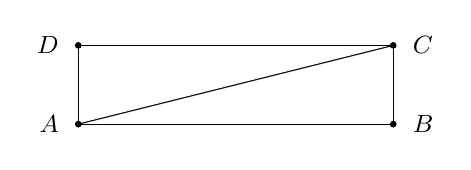
\begin{tikzpicture}[x=10mm,y=10mm,font=\small]
  \draw (1,1) rectangle (5,2);
  \draw (1,1)--(5,2);
  \node [label={[name=label node]left:$A$}] at (1,1) {};
  \node [label={[name=label node]left:$D$}] at (1,2) {};
  \node [label={[name=label node]right:$C$}] at (5,2) {};
  \node [label={[name=label node]right:$B$}] at (5,1) {};

  \foreach \x in {1,5}
    \foreach \y in {1,2}
      \filldraw[fill=black, draw=black]  (\x,\y) circle (1pt);

\end{tikzpicture}

\end{center}

\emph{Dati}: $2 p = 80 \unit{m}$, $\Area = 375\unit{m^2}$.

\emph{Obiettivo}: $\overline {AC}$.


\begin{soluzione}

$\overline {AC} = \sqrt{\overline {AB}^{2} + \overline {BC}^{2}}$ per il teorema 
di Pitagora sul triangolo $ABC$.

Sono incognite le misura dei lati, quindi poniamo $\overline {AB} = x$ e 
$\overline {BC} = y $ con $x > 0$ e $y > 0$.

Il problema si formalizza con il sistema:
$\left\{ \begin{array}{l} x + y = 40 \\x \cdot y = 375 \end{array}\right.$
che esprime la ricerca di due numeri nota la loro somma $40$ e il loro prodotto 
$375$. I numeri richiesti sono le soluzioni reali positive dell'equazione $t^{2} 
- 40 t + 375 = 0$ e precisamente $t_{1} = 15 \vee t_{2} = 25$.

Per come abbiamo disegnato la figura abbiamo quindi: $AB = 25\unit{m}; BC = 
15\unit{m}$ da cui $\overline {AC} = \sqrt{\overline {AB}^{2} + \overline 
{BC}^{2}} =\sqrt{850} = 5 \sqrt{34}\unit{m}$.
\end{soluzione}
% \vspazio\ovalbox{\risolvii \ref{ese:3.81}, \ref{ese:3.82}, \ref{ese:3.83}.}

\begin{problema}
Nel triangolo rettangolo $ABC$, rettangolo in $C$ l'ipotenusa supera il cateto 
maggiore $CB$ di $2\unit{m}$ la differenza tra i cateti è $23\unit{m}$. 
Determinare la misura del perimetro e l'area di $ABC$.
\end{problema}

\begin{multicols}{3}
\emph{Dati}

$\overline {AB} = \overline {CB} + 2$

$\overline {CB} - \overline {AC} = 23$

$A \widehat {C} B = \text{ retto}$.

\emph{Obiettivo}

$2 p$

Area.

 % (c) 2013 Claudio Carboncini - claudio.carboncini@gmail.com
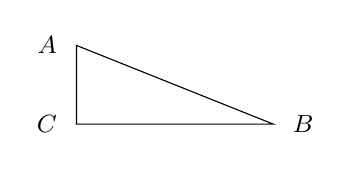
\begin{tikzpicture}[x=10mm,y=10mm,font=\small]

  \draw (1,1) -- (1,2) -- (3.5,1) -- cycle;
  \node [label={[name=label node]left:$A$}] at (1,2) {};
  \node [label={[name=label node]right:$B$}] at (3.5,1) {};
  \node [label={[name=label node]left:$C$}] at (1,1) {};

\end{tikzpicture}

\end{multicols}

\begin{soluzione}

Osserva che $2 p = \overline {AB} + \overline {BC} + \overline {AC}$ e $\Area 
=\frac{\overline {BC} \cdot \overline {AC}}{2}$.
Poni $\overline {BC} = x$ dai dati si ha $\overline {AB} = x + 2$ e 
$\overline{AC} = x - 23$ con
$\left\{\begin{array}{l} x > 0 \text{ essendo misura di un segmento} \\x >23 
\text{ poiché } \overline {AC} \text{ deve essere positiva}
\end{array}\right.$.

Essendo il triangolo rettangolo, i lati sono legati dal teorema di Pitagora
quindi si deve verificare: $\overline {AB}^{2}= \overline {AC}^{2} + \overline 
{BC}^{2}\rightarrow ( x + 2 )^{2} = ( x - 23 )^{2} + x^{2}$. Sviluppando i 
calcoli si ottiene l'equazione risolvente di secondo grado, in forma canonica: 
$x^{2} - 50 x + 525 = 0 \text{ con } \Delta = 400$. L'equazione è determinata 
con il discriminante positivo, quindi esistono due soluzioni reali distinte: 
$x_{1} = 15 \vee x_{2} = 35$ entrambe positive. Ai fini del problema $x_{1} = 
15$ non è accettabile, quindi il problema ha una sola soluzione e $\overline 
{BC} = 35$ $\overline {AB} = 37$ $\overline {AC} = 12$. Conclusione: $2 p = 35 + 
37 + 12 = 84\unit{m}$ $ \Area = 210\unit{m^{2}}$.
\end{soluzione}

\begin{problema}
Un padre aveva $26$ anni alla nascita del figlio; moltiplicando le età attuali 
del padre e del figlio si trova il triplo del quadrato dell'età del figlio; 
calcolare le due età.
\end{problema}
Indichiamo con $p$ l'età attuale del padre e con $f$ l'età del figlio

\emph{Dati}: $p = f + 26;\; p \cdot f = 3 f^{2}$.

\emph{Obiettivo}: $f,\; p$.

\begin{soluzione}
I dati permettono di impostare la relazione $(f + 26) \cdot f = 3 \cdot f^{2}$ 
che esprime il legame tra le età di oggi del padre e del figlio; siamo di
fronte ad un'equazione di secondo grado nell'incognita $f$. La soluzione 
dell'equazione deve essere espressa da un numero positivo poiché esprime l'età.
Risolviamo l'equazione $2 f^{2} - 26 f = 0$ le cui soluzioni sono $f_{1} = 0 
\vee f_{2} = 13$. Per le condizioni poste la soluzione del problema è
$f = 13$. Quindi oggi il figlio ha $13$ anni e il padre $39$ anni.
\end{soluzione}
% % 8<
% \begin{problema}
% Il trapezio isoscele $ABCD$ è inscritto in una semicirconferenza di diametro 
% $AB$ di misura $25\unit{cm}$ determina le misure dei lati del trapezio sapendo 
% che il
% perimetro è $62\unit{cm}$.
% \end{problema}
% 
% \begin{multicols}{2}
% \emph{Dati}
% 
% $\overline {AB} = 25$ $2 p = 62$
% 
% $AB \parallel DC$ $\overline {AD} = \overline {CB}$.
% 
% \emph{Obiettivo}
% 
% $\overline {DC}$ $ \overline {CB}$.
% 
%  % (c) 2013 Claudio Carboncini - claudio.carboncini@gmail.com
\begin{tikzpicture}[x=10mm,y=10mm,font=\small]
  \coordinate(a) at (-2.5,0);
  \coordinate(d) at (120:2.5);
  \coordinate(e) at (90:2.5);
  \coordinate(c) at (60:2.5);
  \coordinate(b) at (2.5,0);
  \coordinate (h) at ($(a)!(c)!(b)$);%trova le coordinate della proiezione di c su a--b
  \draw (-2.5,0) arc (180:0:2.5) -- cycle;% semicirconferenza e diametro
  \draw (a) -- (d) -- (c) -- (b);%disegna il trapezio
  \draw [dotted] (e) -- (0,0);%da E a O
  \draw [dotted] (c) -- (h);% c--h
  \draw [dotted] (e) -- (b);% e--b
  \node [label={[name=label node]below left:$A$}] at (a) {};
  \node [label={[name=label node]below right:$B$}] at (b) {};
  \node [label={[name=label node]above right:$C$}] at (c) {};
  \node [label={[name=label node]above left:$D$}] at (d) {};
  \node [label={[name=label node]above:$E$}] at (e) {};
  \node [label={[name=label node]below:$H$}] at (h) {};
  \filldraw[fill=black, draw=black]  (a) circle (1pt);
  \filldraw[fill=black, draw=black]  (b) circle (1pt);
  \filldraw[fill=black, draw=black]  (c) circle (1pt);
  \filldraw[fill=black, draw=black]  (d) circle (1pt);
  \filldraw[fill=black, draw=black]  (h) circle (1pt);
  \filldraw[fill=black, draw=black]  (e) circle (1pt);

\end{tikzpicture}

% \end{multicols}
% 
% \begin{soluzione}
% $\overline {AB} + \overline {DC} + 2 \overline {BC} = 62$ fissiamo come 
% incognita la misura in cm di $BC$: $\overline {BC} = x$.
% Determiniamo le condizioni sull'incognita: dovrà essere $x > 0$ poiché 
% rappresenta la misura di un segmento e inoltre affinché esista
% realmente il trapezio isoscele il punto $C$ non deve coincidere con il punto 
% medio $E$ dell'arco $DC$ cioè $ CB<EB $, quindi $x < \dfrac{25}{2} \sqrt{2}$.
% 
% Tracciata l'altezza $CH (H \in AB)$ si ha $\overline {DC} = \overline {AB} - 2 
% \overline {HB}$ e per il 1° teorema di Euclide sul triangolo~$ACB$, rettangolo 
% in
% $C$, $\overline {HB}: \overline {CB} = \overline {CB} : \overline{AB}$ 
% determiniamo quindi la misura di $HB$ in funzione dell'incognita fissata:
% $\overline {HB} = \dfrac{x^{2}}{25}$ da cui $\overline {DC} = 25 - \dfrac{2 
% x^{2}}{25}$.
% 
% Costruiamo l'equazione risolvente: $25 + 2 x + 25 - \dfrac{2 x^{2}}{25} = 62 
% \rightarrow x^{2} - 25 x + 150 = 0$ che ha soluzioni $x_{1} = 10 \vee x_{2} = 
% 15$, entrambe accettabili. Si hanno dunque due trapezi inscritti che risolvono 
% il problema.
% \begin{center}
%  % (c) 2013 Claudio Carboncini - claudio.carboncini@gmail.com
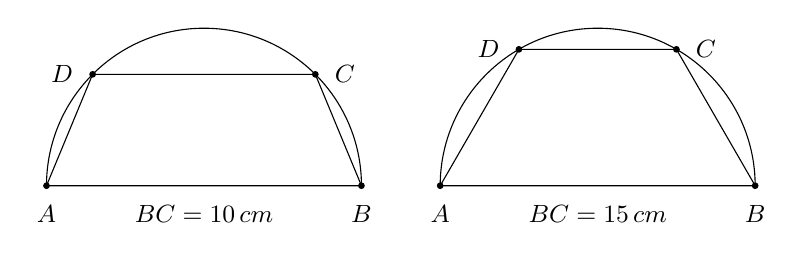
\begin{tikzpicture}[x=10mm,y=10mm,font=\small]
  \coordinate(a) at (-2,0);
  \coordinate(d) at (135:2);
  \coordinate(c) at (45:2);
  \coordinate(b) at (2,0);
  \coordinate(a1) at (3,0);
  \coordinate(d1) at (4,1.732);
  \coordinate(c1) at (6,1.732);
  \coordinate(b1) at (7,0);
  \coordinate(t) at (0,0);
  \coordinate(t1) at (5,0);
  \draw (-2,0) arc (180:0:2) -- cycle;% semicirconferenza e diametro primo trapezio
  \draw (3,0) arc (180:0:2) -- cycle;% semicirconferenza e diametro secondo trapezio
  \draw (a) -- (d) -- (c) -- (b);%disegna il trapezio
  \draw (a1) -- (d1) -- (c1) -- (b1);%disegna il secondo trapezio
  \node [label={[name=label node]below:$A$}] at (a) {};
  \node [label={[name=label node]below:$B$}] at (b) {};
  \node [label={[name=label node]right:$C$}] at (c) {};
  \node [label={[name=label node]left:$D$}] at (d) {};
  \node [label={[name=label node]below:$BC=10\,  cm$}] at (t) {};
  \node [label={[name=label node]below:$A$}] at (a1) {};
  \node [label={[name=label node]below:$B$}] at (b1) {};
  \node [label={[name=label node]right:$C$}] at (c1) {};
  \node [label={[name=label node]left:$D$}] at (d1) {};
  \node [label={[name=label node]below:$BC=15\,  cm$}] at (t1) {};
  \filldraw[fill=black, draw=black]  (a) circle (1pt);
  \filldraw[fill=black, draw=black]  (b) circle (1pt);
  \filldraw[fill=black, draw=black]  (c) circle (1pt);
  \filldraw[fill=black, draw=black]  (d) circle (1pt);
  \filldraw[fill=black, draw=black]  (a1) circle (1pt);
  \filldraw[fill=black, draw=black]  (b1) circle (1pt);
  \filldraw[fill=black, draw=black]  (c1) circle (1pt);
  \filldraw[fill=black, draw=black]  (d1) circle (1pt);

\end{tikzpicture}

% \end{center}
% \end{soluzione}
% % >8
\begin{problema}
Un capitale di $25000$ euro viene depositato in banca a un tasso di interesse 
annuo $c$. Gli interessi maturati durante il primo anno non vengono ritirati.
Nell'anno seguente si investono sia il capitale sia gli interessi maturati a un 
tasso di interesse annuo aumentato dello $0,5\%$. Alla fine dei due anni si 
ritira
la somma di $26291,10$ euro. Calcola i tassi di interesse praticati dalla banca.
\end{problema}
Assumiamo come incognita $c$ il tasso di interesse praticato il primo anno, 
espresso come numero decimale e
non in forma percentuale. Il tasso praticato nel secondo anno sarà $c+0,005$.

\begin{soluzione}
Alla fine del primo anno in banca rimane tra capitale e interessi \[25000 + 
25000 \cdot c = 25000 ( 1 + c ).\] Nel secondo anno il tasso praticato è 
$c+0,005$ che va applicato alla somma $25000(1+c)$. Si~ottiene quindi 
l'equazione \[25000 ( 1 + c ) ( 1 + c + 0,005 ) = 26291,10.\]
Moltiplicando le parentesi tonde si ha $25000 ( 1,005 + c + 1,005 c + c^{2} ) = 
26291,10$ e poi dividendo per $25000$ e ordinando otteniamo
$c^{2} + 2,005 c - 0,046644=0$ con soluzioni
\[c_{1,2}~=~\dfrac{- 2,005 \pm \sqrt{4,020025 + 0,186576}}{2} = \dfrac{-2,005 
\pm 2,051}{2}\Rightarrow c_{1} = - 2,028 \vee c_{2} = 0,023.\]
La soluzione $c_1$ è negativa e non accettabile. La risposta al problema è 
$0,023$ cioè $2,3\%$ il primo anno e $2,8\%$ il secondo anno.
\end{soluzione}
% \vspazio\ovalbox{\risolvii \ref{ese:3.112}, \ref{ese:3.113}, \ref{ese:3.114}, 
% \ref{ese:3.115}, \ref{ese:3.116}, \ref{ese:3.117}, \ref{ese:3.118}, 
% \ref{ese:3.119}, \ref{ese:3.120}, \ref{ese:3.121}, \ref{ese:3.122},}
% 
% \vspazio\ovalbox{\ref{ese:3.123}, \ref{ese:3.124}, \ref{ese:3.125}, 
% \ref{ese:3.126}, \ref{ese:3.127}, \ref{ese:3.128}, \ref{ese:3.129}, 
% \ref{ese:3.130}, \ref{ese:3.131}, \ref{ese:3.132}, \ref{ese:3.133}, 
% \ref{ese:3.134}, \ref{ese:3.135}, \ref{ese:3.136},}
% 
% \vspazio\ovalbox{\ref{ese:3.137}, \ref{ese:3.138}, \ref{ese:3.139}, 
% \ref{ese:3.140}, \ref{ese:3.141}, \ref{ese:3.142}, \ref{ese:3.143}, 
% \ref{ese:3.144}, \ref{ese:3.145}, \ref{ese:3.146}, \ref{ese:3.147}, 
% \ref{ese:3.148}, \ref{ese:3.149}, \ref{ese:3.150}.}
% % 8<
% \subsection{Problemi con un parametro}
% I problemi che abbiamo proposto sono caratterizzati da dati numerici e di 
% conseguenza le soluzioni numeriche dell'equazione risolvente sono facilmente
% confrontabili con le condizioni poste sull'incognita. Abbiamo anche visto che le 
% soluzioni dell'equazione non sempre sono soluzioni del problema e
% può anche succedere che il problema abbia due soluzioni.
% 
% Affrontiamo ora un problema letterale, nel quale alcuni dati sono espressi da 
% lettere. In questi problemi dovremo rispettare le condizioni poste 
% sull'incognita, ma anche analizzare per quali valori della lettera il problema 
% ammette soluzioni reali. Dovremo quindi procedere con la discussione 
% dell'equazione parametrica risolvente per stabilire se il problema letterale 
% ammette soluzioni.
% 
% \begin{problema}
% Sul lato $ a $ dell'angolo $ a \widehat{V} b $ di $ 60\grado $ si fissano i 
% punti $ A $ e $ B $ tali che $ \overline{VA } = 2 k $ e $ \overline {VB} = 8 k 
% $.
% Determina sul lato $ b $ un punto $ P $ in modo che il rapporto tra $ PB $ e $ 
% PA $ sia $ 2 $.
% \end{problema}
% 
% \begin{multicols}{2}
% \emph{Dati}
% 
% $a \widehat{V} b = 60\grado$
% 
% $\overline {VA} = 2 k; \;
%  \overline {VB} = 8 k $.
% 
% \emph{Obiettivo}
% 
% $P \in b \text{ tale che } \dfrac{PB}{PA} = 2$.
% \begin{center}
%  % (c) 2013 Claudio Carboncini - claudio.carboncini@gmail.com
\begin{tikzpicture}[x=10mm,y=10mm,font=\small]

  \coordinate(v) at (0,0);%il vertice dell'angolo
  \coordinate(a) at (60:4);%la retta a
  \coordinate(b) at (4,0);%la retta b
  \coordinate(a1) at (60:0.8);%il punto A
  \coordinate(b1) at (60:3.2);%il punto B
  \coordinate(p) at (3.2,0);%il punto P
  \coordinate (m) at ($(v)!(b1)!(p)$);%trova le coordinate della proiezione di b su v--p
  \coordinate (n) at ($(v)!(a1)!(p)$);%trova le coordinate della proiezione di b su v--p
  \draw (a) -- (v)  -- (b);%disegna l'angolo
  \draw (b1) -- (p);%disegna il segmento b--p
  \draw (a1) -- (p);%disegna il segmento a--p
  \draw [dotted] (a1) -- (n);%perpendicolare da A a b
  \draw [dotted] (b1) -- (m);%perpendicolare da B a b
  \node [label={[name=label node]left:$V$}] at (v) {};
  \node [label={[name=label node]left:$A$}] at (a1) {};
  \node [label={[name=label node]left:$B$}] at (b1) {};
  \node [label={[name=label node]left:$a$}] at (a) {};
  \node [label={[name=label node]below:$P$}] at (p) {};
  \node [label={[name=label node]below:$M$}] at (m) {};
  \node [label={[name=label node]below:$N$}] at (n) {};
  \node [label={[name=label node]above:$b$}] at (b) {};

\end{tikzpicture}

% \end{center}
% 
% \end{multicols}
% \emph{Osservazione preliminare}: le misure dei segmenti $ VA $ e $ VB $ sono 
% espresse in forma letterale, affinché il problema abbia significato deve essere
% $k > 0$.
% 
% \begin{soluzione}
% La posizione del punto $ P $ sul lato $ b $ sarà individuata dalla distanza di $ 
% P $ da $ V $: poniamo quindi $\overline {VP} = x$ con $x > 0$ e determiniamo
% $\overline {PB}$ e $\overline {PA}$ in funzione di $ x $ per poter sfruttare la 
% richiesta contenuta nell'obiettivo come equazione risolvente.
% 
% Sia $ M $ il piede della perpendicolare da $ B $ al lato $ b $ nel triangolo 
% rettangolo $ PMB $ si ha $\overline {PB}^{2} = \overline {BM}^{2} + \overline 
% {PM}^{2}$(*) per il teorema di Pitagora. Nel triangolo $ BVM $, rettangolo in $ 
% M $ con l'angolo $ V $ di $ 60\grado $ si ha $\overline {BM} = \frac{1}{2} 
% \overline {BV} \cdot \sqrt{3} = 4 k\cdot \sqrt{3}$ $\overline {PM} = \overline 
% {VP} - \overline {VM}$ e $\overline {VM} = \frac{1}{2} \overline {VB} = 4 k$ per 
% quanto detto sul triangolo $ BVM $, quindi $\overline {PM} = x - 4 k$ 
% sostituendo in (*) si ottiene $\overline {PB}^{2} = 48 k^{2} + ( x - 4 k )^{2}$.
% 
% Sia $ N $ il piede della perpendicolare da $ A $ al lato $ b $ nel triangolo 
% rettangolo $ PNA $, con analogo ragionamento otteniamo: $\overline {PA}^{2} = 
% \overline {AN}^{2} + \overline {PN}^{2}$ (**) per il teorema di Pitagora. Nel 
% triangolo $ AVN $, rettangolo in $ N $ con l'angolo $ V $ di $ 60\grado $ si ha
% $\overline {AN} = \frac{1}{2} \overline {AV} \cdot \sqrt{3} = k \cdot \sqrt{3}$ 
% $ \overline {VN} = \frac{1}{2} \overline {AV} = k$ e $\overline {PN} = \overline 
% {VP} - \overline {VN} = x - k$ sostituendo in (**) si ottiene $\overline 
% {PA}^{2} = 3 k^{2} + ( x - k )^{2}$.
% 
% Determiniamo l'equazione risolvente ricordando che il rapporto tra due segmenti 
% è uguale al rapporto tra le rispettive misure ed elevando al quadrato
% si ha $\frac{\overline {PB}^{2}}{\overline {PA}^{2}} = 4$. Sostituendo quanto 
% trovato si ottiene l'equazione $48 k^{2} + ( x - 4 k )^{2} = 4 \cdot \left[ 3 
% k^{2} + ( x - k )^{2} \right]$ da cui $x^{2} = 16 k^{2}$. Si tratta di 
% un'equazione di secondo grado pura, avente due soluzioni reali opposte essendo 
% il secondo membro positivo, quindi $x_{1} = - 4 k$ e $x_2=4 k$ per le condizioni 
% poste solo $ x_2 $ è accettabile.
% 
% Con quale punto della figura tracciata inizialmente viene a coincidere il punto 
% $ P $ che risolve il problema?
% \end{soluzione}
% 
% \vspazio
% \ovalbox{\risolvii \ref{ese:3.151}, \ref{ese:3.152}, \ref{ese:3.153}, 
%          \ref{ese:3.154}, \ref{ese:3.155}, \ref{ese:3.156}, \ref{ese:3.157}, 
%          \ref{ese:3.158}, \ref{ese:3.159}}
% \vspazio
% 
% % >8
% 
% HO TOLTO LA SEZIONE CON PROBLEMI PARAMETRICI


\section{L'equazione di terzo grado, un po' di storia}
\label{sec:eq2gr_gradosup}(questa descrizione credo sia da cambiare)

Problema: ``Trovare un numero il cui cubo, insieme con due suoi quadrati e dieci 
volte il numero stesso, dia come somma 20''.

Il problema enunciato venne posto da Giovanni Panormita, astronomo e filosofo 
alla corte di Federico II, a Leonardo Pisano, detto Fibonacci, che ne tentò la 
soluzione nella sua opera Flos.

Con il linguaggio matematico attuale il problema si formalizza nell'equazione di 
terzo grado $x^3+2x^2+10x=20$ Fibonacci pervenne al valore approssimato 
$x=1,3688$ come soluzione al problema, senza indicare la via seguita per la sua 
determinazione. Pur tuttavia egli riuscì a dimostrare che le soluzioni di 
un'equazione di terzo grado non possono mai esprimersi mediante radicali 
quadratici neanche se sovrapposti.

Solo tra il 1540 e il 1545, ad opera dei matematici italiani Niccolò Fontana, 
detto Tartaglia, e Gerolamo Cardano, fu scoperta la formula risolutiva 
dell'equazione generale di terzo grado.

Cardano dimostra che ogni equazione di terzo grado $ax^3+bx^2+cx+d=0$ è 
riconducibile alla forma $y^3+{py}+q=0$. Operando con la sostituzione $x=y-\frac 
b{3a}$ si ricava la formula risolutiva: 
\[y=\sqrt[3]{-\frac q 2+\sqrt{\left(\frac p 3\right)^3+\left(\frac q 
2\right)^2}}+\sqrt[3]{-\frac q 2-\sqrt{\left(\frac p 3\right)^3+\left(\frac q 
2\right)^2}}\] 
da cui poi risale alla soluzione dell'equazione assegnata.
\begin{exrig}
\begin{esempio}
Risolvere l'equazione: $x^3+3x^2+6x+5=0$.

Operiamo la sostituzione $x=y-\frac b{3a}$ che in questo caso è $x=y-1$ 
l'equazione diventa $(y-1)^3+3(y-1)^2+6(y-1)+5=0$ ed eseguendo i calcoli si ha 
$y^3+3y+1=0$ con $p=3$ e~$q=1$.
Applicando la formula risolutiva si ha 
\[y=\sqrt[3]{-\frac 1 2+\sqrt{\frac 1 4+1}}+\sqrt[3]{-\frac 1 2-\sqrt{\frac 1 
4+1}}=\sqrt[3]{\frac{\sqrt 5-1} 2}+\sqrt[3]{\frac{-\sqrt 5-1} 2}\] 
e quindi $x=\sqrt[3]{\dfrac{\sqrt 5-1} 2}+\sqrt[3]{\dfrac{-\sqrt 5-1} 2}-1$.
\end{esempio}

\begin{esempio}
Risolvere l'equazione $x^3=15x+4$ applicando la formula di Cardano.

Notiamo che è $p=-15$ e $q=-4$ e dunque sotto la radice quadrata della formula 
si ha $\left(\frac p 3\right)^3+\left(\frac q 2\right)^2=(-5)^3+(-2)^2=-121$ 
pertanto non un numero
reale, mentre è evidente la soluzione reale $x=4$. Questa circostanza ha spinto 
il 
matematico Raffaele Bombelli, ad elaborare nella sua opera ``Algebra'' del 1572, 
calcoli con radici 
quadrate di numeri negativi (numeri) che troveranno una sistemazione coerente 
nella teoria dei 
numeri complessi sviluppata da Fiedrich Gauss.

Vediamo come possiamo determinare l'I.S. dell'equazione di Bombelli con le 
nostre conoscenze. Scriviamo l'equazione nella forma canonica $p(x)=0\Rightarrow 
x^3-15x-4=0$ sappiamo che uno zero intero è $x=4$ dunque scomponiamo dividendo 
$p(x)=x^3-15x-4$ per il binomio $x-4$. Potete verificare che si ottiene 
$x^3-15x-4=(x-4)\cdot (x^2+4x+1)=0$ da cui, per la legge di annullamento del 
prodotto, 
\[x-4=0\Rightarrow x=4\vee x^2+4x+1=0\Rightarrow x_{1,2}=-2\pm \sqrt 3.\]

Poco dopo la scoperta della formula risolutiva per le equazioni di terzo grado 
il matematico italiano Ferrari trovò anche la formula per risolvere le 
equazioni di quarto grado. 
Le ricerche per trovare la formula che risolvesse l'equazione di quinto grado 
furono invece vane, non perché i matematici non furono abbastanza 
``ingegnosi'' bensì per il fatto che, come dimostrò Galois non esistono 
formule che per mezzo di radici ed altre operazioni algebriche possano 
risolvere le equazioni dal quinto grado in poi. In altre parole esistono 
solo formule per le equazioni di secondo, terzo e quarto grado.

Oggigiorno, tuttavia, si preferisce non approfondire le applicazioni di queste 
formule. Si usa applicare solo la formula risolutiva per le equazioni di secondo 
grado e per quelle di grado superiore al secondo si applicano i metodi 
algebrici che vedremo solo parzialmente in questo capitolo e che completeremo 
nel prossimo volume  oppure si preferisce applicare metodi di calcolo 
numerico che danno le soluzioni per approssimazioni successive.
\end{esempio}
\end{exrig}

\section{Equazioni riconducibili al prodotto di due o più fattori}
\label{sec:eq2gr_scomponibili}

In questo capitolo ci proponiamo di descrivere uno dei metodi algebrici per 
determinare l'Insieme Soluzione di equazioni algebriche di grado superiore 
al secondo.

Ricordiamo che un'equazione algebrica si presenta nella forma $p(x)=0$ dove 
$p(x)$ è un polinomio nella variabile $x$, di grado $n$, a coefficienti reali: 
\[a_nx^n+a_{n-1}x^{n-1}+ \ldots +a_2x^2+a_1x+a_0=0.\]

\begin{exrig}
\begin{esempio}
Determinare le radici reali dell'equazione $4x^3+x^2-4x-1=0$.

Scomponiamo in fattori il polinomio al primo membro mediante raccoglimento 
parziale: 
\[p(x)=4x^3+x^2-4x-1=4x \left(x^2-1\right)+\left(x^2-1\right)=\left(x^2-1\right) 
(4x+1).\] 
Per la legge dell'annullamento del prodotto si ottiene 
\[x^2-1=0\vee 4x+1=0 \Rightarrow x^2-1=0\Rightarrow x_1=-1\vee x_2=1\text{ e 
}4x+1=0\Rightarrow x=-\frac{1}{4}.\] L'equazione ha dunque tre soluzioni reali 
distinte e $\IS=\left\{-1;1;-\frac 1 4\right\}$.
\end{esempio}
\begin{esempio}
Determinare le radici reali dell'equazione fratta 
$\frac{2x+3}{2x+1}+\frac{x^2}{x+1}=5x+3$.

Riduciamo allo stesso denominatore 
\[\frac{2x^2+5x+3+2x^3+x^2-10x^3-15x^2-5x-6x^2-9x-3}{(2x+1)\cdot (x+1)}=0.\]
Poniamo le Condizioni d'Esistenza $x\neq -\frac 1 2\wedge x\neq -1$. Eliminiamo 
il denominatore e sommiamo i monomi simili; otteniamo un'equazione di terzo 
grado $8x^3+18x^2+9x=0$. Scomponiamo in fattori il polinomio $x\cdot 
\left(8x^2+18x+9\right)=0$. Per la legge di annullamento $x=0\vee x^2+18x+9=0$. 
Risolvendo anche l'equazione di secondo grado con la formula risolutiva si 
ottengono le soluzioni $x_1=0\vee x_2=-\frac 3 4\vee x_3=-\frac 3 2$.

\osservazione
Si dimostra che un'equazione ammette tante soluzioni, che possono essere reali e 
distinte, coincidenti o non reali, quante ne indica il suo grado.

Ricordiamo che uno zero di un polinomio è il valore che assegnato alla variabile 
rende il polinomio uguale a zero. L'obiettivo posto viene raggiunto ponendo il 
polinomio uguale a zero, come nell'esempio seguente.
\end{esempio}

\begin{esempio}
Trovare gli zeri del seguente polinomio di terzo grado $p(x)=x^3-7x^2+4x+12$.

Scriviamo l'equazione $x^3-7x^2+4x+12=0$ e cerchiamo di scomporre con il metodo 
di Ruffini. Sostituendo $x=-1$ si ottiene $(-1)^3-7(-1)^2+4(-1)+12=-1-7-4+12=0$. 
Possiamo allora dividere il polinomio $x^3-7x^2+4x+12=0$ per il binomio $x+1$. 
Applicando la regola di Ruffini si ha:
\begin{center}
% (c) 2013 Claudio Carboncini - claudio.carboncini@gmail.com

\begin{tikzpicture}[x=5mm,y=5mm]
\matrix (a)[matrix of nodes, nodes in empty cells,nodes={ text width=8mm, text depth=1mm, text centered}]{
&$1$&$-7$&$4$&$ 12 $\\
$ -1 $&&$ -1 $&$ 8 $&$-12$\\
&$ 1 $&$ -8 $&$12$&//\\
};  
\begin{scope}[blue]
\draw(a-1-2.north west)--(a-3-1.south east);
\draw(a-2-1.south west)--(a-2-5.south east);
\draw(a-1-4.north east)--(a-3-4.south east);
      \end{scope}
\end{tikzpicture}

\end{center}
Il polinomio si scompone in $(x+1)(x^2-8x+12)$. Per la legge di annullamento del 
prodotto $x+1=0\vee x^2-8x+12=0$. L'equazione $x+1=0$ dà come soluzione $x=-1$. 
L'equazione $x^2-8x+12=0$ si può risolvere con la formula risolutiva ridotta 
$x_{1,2}=4\pm \sqrt{16-12}=4\pm 2$. Il polinomio assegnato ha tre zeri distinti 
$x_1=-1\vee x_2=2\vee x_3=6$.
\end{esempio}
\end{exrig}

% \ovalbox{\risolvii \ref{ese:5.1}, \ref{ese:5.2}, \ref{ese:5.3}, \ref{ese:5.4}, 
% \ref{ese:5.5}, \ref{ese:5.6}, \ref{ese:5.7}, \ref{ese:5.8}, \ref{ese:5.9}, 
% \ref{ese:5.10}, \ref{ese:5.11}}

Altre tipologie di equazioni di grado superiore al II saranno trattate il 
prossimo anno.

\section{Sistemi di secondo grado}
\label{sec:eq2gr_sistemi}

Ricordiamo che un sistema di equazioni non è altro che l'insieme di più 
equazioni con le stesse incognite. L'insieme delle soluzioni è dato 
dall'intersezione degli insiemi delle soluzioni delle singole equazioni.

\begin{definizione}
Il \emph{grado di un sistema di equazioni}, se le equazioni che formano il 
sistema sono costituite da polinomi, è dato dal prodotto dei gradi delle 
equazioni che lo compongono.
\end{definizione}

\begin{exrig}
\begin{esempio}
Determinare il grado dei seguenti sistemi di equazioni

\begin{itemize}
\item $\left\{\begin{array}{l}-2x+3y=4 \\3x+5y-2=0\end{array}\right.$ entrambe 
le equazioni sono di primo grado; il sistema è di primo grado;
\item $\left\{\begin{array}{l}2x-y=0 \\x^2+6y^2-9=0\end{array}\right.$ la prima 
equazione è di primo grado, la seconda di secondo grado; il sistema è di secondo 
grado;
\item $\left\{\begin{array}{l}x^2+y^2=0 \\y=3x^2-2x+6=0\end{array}\right.$ 
entrambe le equazioni sono di secondo grado; il sistema è di quarto grado.
\end{itemize}
\end{esempio}
\end{exrig}
I sistemi di secondo grado sono dunque composti da un'equazione di secondo grado 
e da una di primo grado.

\subsection{Sistemi di secondo grado numerici}
\begin{exrig}
\begin{esempio}
Risolvere il seguente sistema 
$\left\{\begin{array}{l}{2x-y=0}\\{x^2+6y^2-9=0}\end{array}\right..$

Utilizziamo il metodo di sostituzione che abbiamo già visto per i sistemi di 
primo grado.
\begin{itemize*}
\item Ricaviamo una delle due incognite dall'equazione di primo grado e 
sostituiamo nell'equazione di secondo grado:
\[\left\{\begin{array}{l}y=2x \\
x^2+6\cdot (2x)^2-9=0\end{array}\right. 
\Rightarrow\left\{\begin{array}{l}y=2x \\
x^2+24x^2-9=0\end{array}\right. 
\Rightarrow \left\{\begin{array}{l}y=2x \\
25x^2-9=0\end{array}\right.;\]
\item risolviamo l'equazione di secondo grado in una sola incognita. Questa 
equazione è detta equazione risolvente del sistema:
 $25x^2-9=0\Rightarrow x_1=-\frac 3 5\vee x_2=\frac 3 5$
\item Si sostituiscono i valori trovati per la $ x $ nella equazione di primo 
grado per trovare i valori corrispondenti della $ y $. Le coppie $(x_1;y_1)$ e 
$(x_2;y_2)$ se ci sono, si dicono soluzioni del sistema.
\[\left\{\begin{array}{l}{y=2x}\\
{25x^2-9=0}\end{array}\right. 
\Rightarrow \left\{\begin{array}{l}x_1=-\frac 3 5 \\
y_1=2\cdot \left(-\frac 3 5\right)=-\frac 6 5\end{array}\right.\vee 
\left\{\begin{array}{l}x_2=+\frac 3 5 \\
y_2=2\cdot \left(\frac 3 5\right)=+\frac 6 5 \end{array}\right.\] 
quindi con soluzioni 
\[\left(-\frac 3 5;-\frac 6 5\right)\vee \left(\frac 3 5;\frac 6 5\right).\]
\end{itemize*}

\begin{multicols}{2}
Le soluzioni del sistema possono essere interpretate geometricamente come i 
punti di intersezione tra la retta rappresentata dall'equazione $y=2x$ e la 
curva rappresentata dall'equazione $x^2+6y^2=9$. Con qualsiasi software che 
disegni grafici inseriamo le due equazioni e otteniamo la seguente figura.
La curva rappresentata dalla seconda equazione è una ellisse; i punti $ A $ e $ 
B $, intersezione tra retta ed ellisse, corrispondono alle soluzioni del 
sistema.
\begin{center}
% (c) 2013 Claudio Carboncini - claudio.carboncini@gmail.com
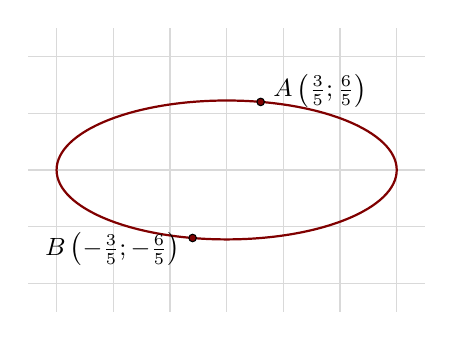
\begin{tikzpicture}[x=8mm, y=8mm,font=\small,scale=.9]
\draw[step=0.8cm,color=gray!30] (-3.5,-2.5) grid (3.5,2.5);
  \tkzInit[xmin=-3.5,xmax=3.5,ymin=-2.5,ymax=2.5]
  \begin{scope}[font=\small]
    \tkzAxeY[orig = false, label options={left = 1pt}]
    \tkzAxeX[orig = true, label options={below = 1pt}]
  \end{scope}
  \tkzFct[domain=-2:2,thick,color=blue]{2*x};

\draw[thick,color=Maroon] (0,0) ellipse (3 and 1.225);
%il punto A
\draw[fill=Maroon] (.6,1.2)circle (1.5pt);
\node[right] at (.65,1.4) {$A \left(\frac{3}{5};\frac{6}{5}\right)$};
%il punto B
\draw[fill=Maroon] (-.6,-1.2)circle (1.5pt);
\node[left] at (-.65,-1.4) {$B \left(-\frac{3}{5};-\frac{6}{5}\right)$};

\end{tikzpicture}

\end{center}
 \end{multicols}
\end{esempio}

\begin{esempio}
Risolvere il seguente sistema: $\left\{\begin{array}{l}x-y=-2 
\\x^2+y-3x-1=0\end{array}\right..$

Isoliamo la $y$ dell'equazione di primo grado e sostituiamo nell'equazione di 
secondo grado 
\[\left\{\begin{array}{l}y=x+2 \\
x^2+\left(x+2\right)-3x-1=0\end{array}\right. 
\Rightarrow\left\{\begin{array}{l}y=x+2 \\
x^2-2x+1=0\end{array}\right.\]

L' \emph{equazione risolvente del sistema}. $x^2-2x+1=0$ ha il discriminante 
uguale a zero e due soluzioni reali coincidenti: $x_1=x_2=1$.

Il sistema ha due soluzioni reali coincidenti, 
\[\left\{\begin{array}{l}y=x+2 \\x^2-2x+1=0\end{array}\right. 
\Rightarrow\left\{\begin{array}{l}x=1 \\
y=1+2=3\end{array}\right.\] 
quindi con soluzione $(1;3)$.
\begin{multicols}{2}
Con qualsiasi software che disegni grafici inseriamo le due equazioni e 
otteniamo la seguente figura.
La curva rappresentata dalla seconda equazione è una parabola.Le soluzioni del 
sistema possono allora essere interpretate geometricamente come i punti di 
incontro tra la retta rappresentata dall'equazione $y=x+2$ e la parabola 
rappresentata dall'equazione $y=-x^2+3x+1$. La soluzioni saranno due punti reali 
coincidenti. 

Questo punto è detto punto di tangenza tra retta e parabola.
\begin{center}
% (c) 2013 Claudio Carboncini - claudio.carboncini@gmail.com
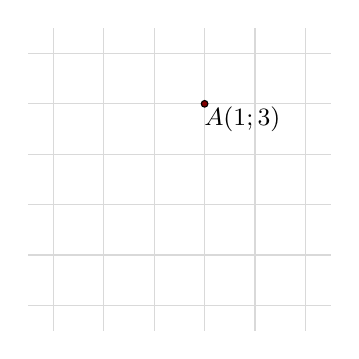
\begin{tikzpicture}[x=8mm, y=8mm,font=\small,scale=.8]
\draw[step=0.8cm,color=gray!30] (-2.5,-1.5) grid (3.5,4.5);
  \tkzInit[xmin=-2.5,xmax=3.5,ymin=-1.5,ymax=4.5]
  \begin{scope}[font=\small]
    \tkzAxeY[orig = false, label options={left = 1pt}]
    \tkzAxeX[orig = true, label options={below = 1pt}]
  \end{scope}
\tkzFct[domain=-.5:3.5,thick,color=Maroon]{-x*x+3*x+1};
\tkzFct[domain=-3.5:6.5,thick,color=blue]{x+2};
%il punto A
\node[right] at (0.8,2.7) {$A (1;3)$};
\draw[fill=Maroon] (1,3)circle (1.5pt);
\end{tikzpicture}

\end{center}
 \end{multicols}
\end{esempio}

\begin{esempio}
Risolvere il seguente sistema: $\left\{\begin{array}{l}x^2+y^2=4 
\\3x+4y=12\end{array}\right..$

Isoliamo $y$ nell'equazione di primo grado e sostituiamola nell'equazione di 
secondo grado 
\[\left\{\begin{array}{l}y=-\frac 3 4x+3 \\
x^2+\left(-\frac 3 4x+3\right)^2-4=0\end{array}\right. 
\Rightarrow\left\{\begin{array}{l}y=-\frac 3 4x+3 \\
x^2+\frac 9{16}x^2-\frac 9 2x+9-4=0\end{array}\right. 
\Rightarrow\left\{\begin{array}{l}y=-\frac 3 4x+3 \\
\frac{25}{16}x^2-\frac{9}{2}x+5=0\end{array}\right..\]

Risolviamo l'equazione di secondo grado in una sola incognita 
$\frac{25}{16}x^2-\frac 9 2x+5=0$ e verifichiamo che $\Delta =\frac{81} 
4-\frac{125} 4$ è negativo, quindi l'equazione non ha soluzioni reali e 
$\IS=\emptyset $. Il sistema non ha soluzioni reali e si dice 
\emph{impossibile}.

\begin{multicols}{2}
Le soluzioni del sistema possono essere interpretate geometricamente come i 
punti di incontro tra la retta rappresentata dall'equazione $y=-\frac 3 4x+3$ e 
la curva rappresentata dall'equazione $x^2+y^2=4$. Nella rappresentazione 
grafica ottenuta con un software che disegna grafici le figure geometriche 
ottenute non hanno punti d'incontro.
La curva rappresentata dalla prima equazione è una circonferenza; retta e 
circonferenza non hanno punti di intersezione.
\begin{center}
% (c) 2013 Claudio Carboncini - claudio.carboncini@gmail.com
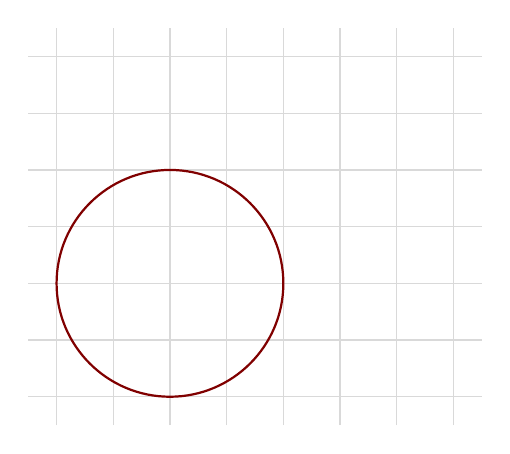
\begin{tikzpicture}[x=8mm, y=8mm,font=\small,scale=.9]
\draw[step=0.8cm,color=gray!30] (-2.5,-2.5) grid (5.5,4.5);
  \tkzInit[xmin=-2.5,xmax=5,ymin=-2.5,ymax=4]
  \begin{scope}[font=\small]
    \tkzAxeY[orig = false, label options={left = 1pt}]
    \tkzAxeX[orig = true, label options={below = 1pt}]
  \end{scope}
\tkzFct[domain=-3:5.5,thick,color=blue]{-0.75*x+3};

\draw[thick,color=Maroon] (0,0) circle (2);
\end{tikzpicture}

\end{center}
 \end{multicols}
\end{esempio}
\end{exrig}

\conclusione
Un sistema di secondo grado, con equazione risolvente di secondo grado, 
rappresenta sempre l'intersezione tra una retta e una curva di secondo grado 
(circonferenza, parabola, ellisse o iperbole). Le soluzioni del sistema 
rappresentano i punti di incontro tra retta e curva. In base al segno del 
discriminante dell'equazione risolvente abbiamo:
\begin{itemize*}
\item $\Delta >0$ le soluzioni del sistema sono le coordinate di due punti 
distinti;
\item $\Delta =0$ le soluzioni del sistema sono le coordinate di due punti 
coincidenti;
\item $\Delta <0$ il sistema non ha soluzioni reali. Retta e curva non hanno 
punti in comune.
\end{itemize*}
\begin{center}
% (c) 2013 Claudio Carboncini - claudio.carboncini@gmail.com
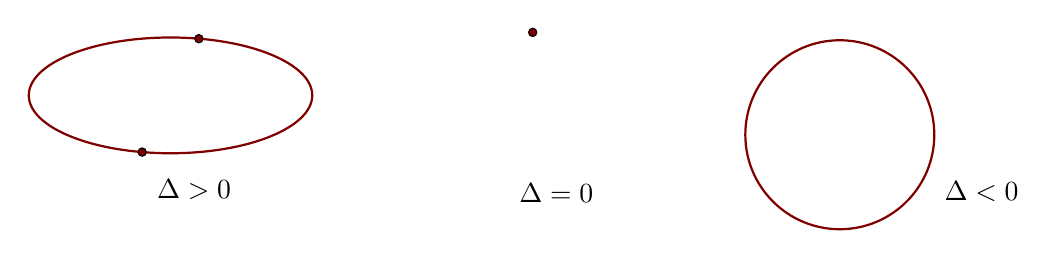
\begin{tikzpicture}[x=6mm, y=6mm]
  \tkzInit[xmin=-3.5,xmax=3.5,ymin=-2.5,ymax=2.5]
  \tkzFct[domain=-2:2,thick,color=blue]{2*x};
\draw[thick,color=Maroon] (0,0) ellipse (3 and 1.225);
\draw[fill=Maroon] (.6,1.2)circle (1.5pt);
\draw[fill=Maroon] (-.6,-1.2)circle (1.5pt);
\node[color =black] at (.5,-2) {$\Delta>0$};

\begin{scope}[xshift=4cm,yshift=-1cm]
\tkzInit[xmin=-2.5,xmax=3.5,ymin=-1.5,ymax=4.5]
\tkzFct[domain=-.5:3.5,thick,color=Maroon]{-x*x+3*x+1};
\tkzFct[domain=-3.5:6.5,thick,color=blue]{x+2};
\draw[fill=Maroon] (1,3)circle (1.5pt);
\node[color =black] at (1.5,-0.4) {$\Delta=0$};
\end{scope}

\begin{scope}[xshift=8.5cm,yshift=-.5cm]
\tkzInit[xmin=-2.5,xmax=5,ymin=-2.5,ymax=4];
\tkzFct[domain=-3:5.5,thick,color=blue]{-0.75*x+3};
\draw[thick,color=Maroon] (0,0) circle (2);
\node[color =black] at (3,-1.2) {$\Delta<0$};
\end{scope}


\end{tikzpicture}

\end{center}

Se l'equazione risolvente risulta essere una equazione di \emph{primo grado} o 
una \emph{uguaglianza} vera o falsa, allora:
\begin{itemize*}
\item se si ottiene una uguaglianza vera, il sistema è indeterminato;
\item se si ottiene una uguaglianza falsa il sistema è impossibile;
\item se l'equazione risolvente è di primo grado determinata, da essa si ricava 
il valore dell'incognita e si sostituisce tale valore nell'altra equazione. Il 
sistema ha una sola soluzione (in questo caso non si parla di due soluzioni 
coincidenti, come nel caso precedente di $\Delta =0$).
\end{itemize*}
\begin{exrig}
\begin{esempio}
Risolvere il sistema 
$\left\{\begin{array}{l}x^2-y^2=0\\x+y=0\end{array}\right.$.

Isoliamo la $y$ dell'equazione di primo grado e sostituiamo nell'equazione di 
secondo grado. 
\[\left\{\begin{array}{l}y=-x \\
x^2-(-x)^2=0\end{array}\right.\ 
\Rightarrow\left\{\begin{array}{l}y=-x \\
x^2-x^2=0\end{array}\right. 
\Rightarrow\left\{\begin{array}{l}y=-x\\
0=0\end{array}\right..\]

L'\emph{equazione risolvente del sistema} in questo caso è una \emph{identità} 
(uguaglianza vera) e tutte le coppie formate da numeri opposti (la prima 
equazione ci vincola ad avere $y=-x$ ) sono soluzioni del sistema: $\forall k\in 
\mathbb{R}\Rightarrow {I.S.}=(k;-k)$. Il sistema ha infinite coppie di numeri 
reali che lo soddisfano e si dice \emph{indeterminato}.
\begin{multicols}{2}
La figura è quella che otteniamo se inseriamo le due equazioni in un software 
che disegna funzioni. La curva di secondo grado è formata dalle due rette 
$x+y=0$ e $x-y=0$ e la seconda equazione rappresenta la retta a che si 
sovrappone alla precedente.
\begin{center}
% (c) 2013 Claudio Carboncini - claudio.carboncini@gmail.com

\begin{tikzpicture}[x=6mm, y=6mm,font=\small,scale=.7]
\draw[step=0.6cm,color=gray!30] (-4.5,-4.5) grid (4.5,4.5);
  \tkzInit[xmin=-4.5,xmax=4.5,ymin=-4.5,ymax=4.5]
  \begin{scope}[font=\small]
    \tkzAxeY[orig = false, label options={left = 1pt}]
    \tkzAxeX[orig = true, label options={below = 1pt}]
  \end{scope}
    \tkzFct[domain=-4.5:4.5,thick,color=blue]{x};
    \tkzFct[domain=-4.5:4.5,very thick,color=Maroon]{-x};
\end{tikzpicture}

\end{center}
\end{multicols}
\end{esempio}

\begin{esempio}
Risolvere il sistema $\left\{\begin{array}{l}\frac 3 
2x+y=0\\x^2-y^2=4\end{array}\right..$

Isoliamo la $y$ dell'equazione di primo grado e sostituiamo nell'equazione di 
secondo grado 
\[\left\{\begin{array}{l}y=-\frac 3 2x \\
x^2-\left(-\frac 3 2x\right)^2=4\end{array}\right.
\Rightarrow \left\{\begin{array}{l}y=-\frac 3 2x \\
x^2-\frac 9 4x^2=4\end{array}\right.
\Rightarrow \left\{\begin{array}{l}y=-\frac 3 2x\\
-\frac 5 4x^2=4\end{array}\right..\]

L'equazione risolvente del sistema $-\frac 5 4x^2=4$ non ha soluzioni, quindi il 
sistema è \emph{impossibile}.
\begin{multicols}{2}
La figura è quella che otteniamo se inseriamo le due equazioni in un software 
che disegna il grafico delle funzioni. 
L'equazione di secondo grado rappresenta una curva detta iperbole e la seconda 
equazione rappresenta la retta; vediamo che curva e retta non hanno punti di 
intersezione.
\begin{center}
% (c) 2013 Claudio Carboncini - claudio.carboncini@gmail.com
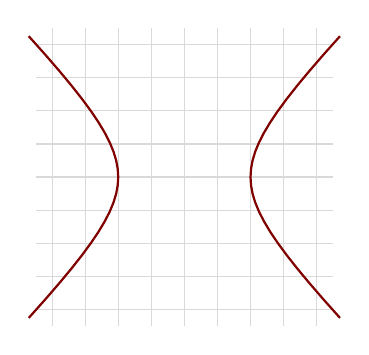
\begin{tikzpicture}[x=6mm, y=6mm,font=\small,scale=.7]
\draw[step=0.6cm,color=gray!30] (-4.5,-4.5) grid (4.5,4.5);
  \tkzInit[xmin=-4.5,xmax=4.5,ymin=-4.5,ymax=4.5]
  \begin{scope}[font=\small]
    \tkzAxeY[orig = false, label options={left = 1pt}]
    \tkzAxeX[orig = true, label options={below = 1pt}]
  \end{scope}
   \pgfmathsetmacro{\e}{1.41421}   % eccentricity
    \pgfmathsetmacro{\a}{2}
    \pgfmathsetmacro{\b}{(\a*sqrt((\e)^2-1)} 
    \draw[thick,color=Maroon] plot[domain=-1.5:1.5] ({\a*cosh(\x)},{\b*sinh(\x)});
    \draw[thick,color=Maroon] plot[domain=-1.5:1.5] ({-\a*cosh(\x)},{\b*sinh(\x)});
    \tkzFct[domain=-4:4,thick,color=blue]{-1.5*x};
\end{tikzpicture}

\end{center}
\end{multicols}
\end{esempio}

\begin{esempio}
Risolvere il sistema 
$\left\{\begin{array}{l}x^2-y^2=4\\-x+y=-1\end{array}\right.$.

Isoliamo la $y$ dell'equazione di primo grado e sostituiamo nell'equazione di 
secondo grado 
\[\left\{\begin{array}{l}y=x-1 \\
x^2-(x-1)^2-4=0\end{array}\right.
\Rightarrow \left\{\begin{array}{l}y=x-1 \\
x^2-x^2+2x-1-4=0\end{array}\right.
\Rightarrow \left\{\begin{array}{l}y=x-1\\2x=5\end{array}\right..\]

L'\emph{equazione risolvente del sistema} in questo caso è l'equazione di primo 
grado $2x-5=0$, la cui soluzione è $x=\frac 5 2$. Si sostituisce il valore 
trovato nell'altra equazione e troviamo la soluzione del sistema che in questo 
caso è unica: 
\[\left\{\begin{array}{l}y=x-1 \\2x=5\end{array}\right. 
\Rightarrow\left\{\begin{array}{l}x=\frac 5 2 \\
y=\frac 5 2-1=\frac 3 2\end{array}\right.\] 
quindi con soluzione \[\left(\frac 5 2;\frac 3 2\right).\]

\begin{multicols}{2}
La figura è quella che otteniamo se inseriamo le due equazioni in un applicativo 
che disegna il grafico di funzioni. L'equazione di secondo grado rappresenta 
una curva detta iperbole e la seconda equazione rappresenta una retta; 
vediamo che curva e retta hanno un solo punto di intersezione.
\begin{center}
% (c) 2013 Claudio Carboncini - claudio.carboncini@gmail.com
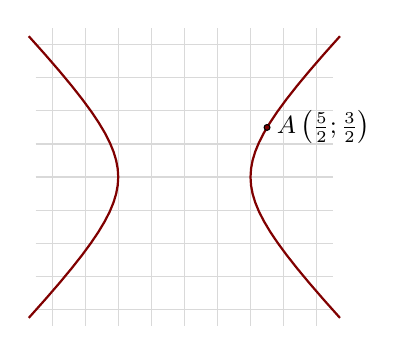
\begin{tikzpicture}[x=6mm, y=6mm,font=\small,scale=.7]
\draw[step=0.6cm,color=gray!30] (-4.5,-4.5) grid (4.5,4.5);
  \tkzInit[xmin=-4.5,xmax=4.5,ymin=-4.5,ymax=4.5]
  \begin{scope}[font=\small]
    \tkzAxeX[below = 3pt]
    \tkzAxeY[left = 1pt]
  \end{scope}
   \pgfmathsetmacro{\e}{1.41421}   % eccentricity
    \pgfmathsetmacro{\a}{2}
    \pgfmathsetmacro{\b}{(\a*sqrt((\e)^2-1)} 
    \draw[thick,color=Maroon] plot[domain=-1.5:1.5] ({\a*cosh(\x)},{\b*sinh(\x)});
    \draw[thick,color=Maroon] plot[domain=-1.5:1.5] ({-\a*cosh(\x)},{\b*sinh(\x)});
    \tkzFct[domain=-4:5,thick,color=blue]{x-1};
    \node[right] at (2.5,1.5) {$A \left(\frac 5 2;\frac 3 2\right)$};
    \draw[fill=Maroon] (2.5,1.5)circle (1.5pt);
\end{tikzpicture}

\end{center}
\end{multicols}
\end{esempio}
\end{exrig}
% \ovalbox{\risolvii \ref{ese:6.1}, \ref{ese:6.2}, \ref{ese:6.3}, \ref{ese:6.4}, 
% \ref{ese:6.5}, \ref{ese:6.6}, \ref{ese:6.7}.}
% % 8<
% \subsection{Sistemi di secondo grado letterali}
% \begin{exrig}
% \begin{esempio}
% Discutere e risolvere il seguente sistema: 
% $\left\{\begin{array}{l}y-kx=-2\\y-x^2=2\end{array}\right.$.
% 
% Si risolve come nel caso degli analoghi sistemi numerici. Bisognerà, 
% nell'equazione risolvente, discutere per quali valore del parametro si 
% otterranno soluzioni reali. Ricaviamo la y dalla prima equazione e sostituiamo 
% nella seconda equazione:
% \[ \left\{\begin{array}{l}y=kx-2\\kx-2-x^2=2\end{array}\right.\ 
% \Rightarrow\left\{\begin{array}{l}y=kx-2\\-x^2+kx-4=0\end{array}\right.\ 
% \Rightarrow\left\{\begin{array}{l}y=kx-2\\x^2-kx+4=0\end{array}\right.. \]
% 
% Discutiamo e risolviamo l'equazione di secondo grado 
% \[ \Delta =k^2-16 \Rightarrow
% \begin{array}{l}\Delta >0\Rightarrow k<-4\vee k>4\Rightarrow 
% x_1=\frac{k-\sqrt{k^2-16}} 2\vee x_2=\frac{k+\sqrt{k^2-16}} 2\\
% \Delta =0\Rightarrow k=-4\vee k=4\Rightarrow x_1=x_2=\frac k 2 \\
% \Delta <0\Rightarrow -4<k<4\Rightarrow \IS=\emptyset \end{array}. \]
% 
% Ricaviamo i valori della x che sostituiamo nella prima equazione: \[ 
% \left\{\begin{array}{l}y-kx=-2\\y-x^2=2\end{array}\right.\text{ se }k\le -4\vee 
% k\ge 4\Rightarrow \left\{\begin{array}{l}x_1=\frac{k-\sqrt{k^2-16}} 2 
% \\y_1=\frac{k^2-4-k\sqrt{k^2-16}} 2\end{array}\right.\vee 
% \left\{\begin{array}{l}x_2=\frac{k+\sqrt{k^2-16}} 2 
% \\y_2=\frac{k^2-4+k\sqrt{k^2-16}} 2\end{array}\right.. \]
% \end{esempio}
% \end{exrig}
% \ovalbox{\risolvii \ref{ese:6.8}, \ref{ese:6.9}.}
% % >8
% \subsection{Sistemi frazionari}
% Si dice frazionario un sistema in cui almeno una delle equazioni che lo 
% compongono è frazionaria; per questo motivo occorre procedere alla definizione 
% del Dominio in cui si ricercano le soluzioni del sistema.
% 
% \begin{exrig}
% \begin{esempio}
% Risolvere il seguente sistema $\left\{\begin{array}{l}2x-y=2 \\\frac 
% x{y+2}=\frac x{2y+5}\end{array}\right.$.
% 
% Determiniamo le condizioni di esistenza di $ \frac x{y+2}=\frac x{2y+5} $:\; 
% $\CE y\neq -2\wedge y\neq -\frac 5 2$.
% 
% Trasformiamo l'equazione frazionaria nella sua forma canonica di equazione 
% intera:
% \begin{align*}
%  &\frac x{y+2}=\frac x{2y+5}\\
% \Rightarrow & x\cdot (2y+5)-x\cdot (y+2)=0\\
% \Rightarrow & 2{xy}+5x-{xy}-2x=0\\
% \Rightarrow & xy+3x=0.
% \end{align*}
% 
% Il sistema diventa: 
% \[\left\{\begin{array}{l}y=2x-2\\
% xy+3x=0\end{array}\right.
% \Rightarrow \left\{\begin{array}{l}y=2x-2\\
% x(2x-2)+3x=0\end{array}\right.
% \Rightarrow \left\{\begin{array}{l}y=2x-2\\
% 2x^2+x=0\end{array}\right..\]
% 
%  $2x^2+x=0$ è l'equazione risolvente; ha soluzioni $x_1=0\vee x_2=-\frac 1 2$.
% 
% Sostituiamo le soluzioni trovate nell'equazione di primo grado e otteniamo le 
% soluzioni del sistema: 
% \[\left\{\begin{array}{l}x_1=0 \\
% y_1=-2\end{array}\right.\vee 
% \left\{\begin{array}{l}x_2=-\frac 1 2\\
% y_2=-3\end{array}\right. 
% \Rightarrow\left(0;-2\right)\vee \left(-\frac 1 2;-3\right).\]
% 
% La soluzione $(0;-2)$ non soddisfa le $\CE$ Il sistema ha soluzione 
% $\left(-\frac 1 2;-3\right)$.
% \end{esempio}
% \end{exrig}
% % \ovalbox{\risolvii \ref{ese:6.10}, \ref{ese:6.11}}
% 
% \subsubsection{Sistemi di secondo grado in tre incognite}
% Quanto detto si può estendere ai sistemi di secondo grado di tre o più equazioni 
% con altrettante incognite. Per risolvere uno di tali sistemi si cercherà, 
% operando successive sostituzioni a partire dalle equazioni di primo grado, di 
% ottenere un'equazione di secondo grado in una sola incognita (equazione 
% risolvente del sistema).
% 
% A partire dalle eventuali soluzioni di tale equazione, si determineranno poi le 
% soluzioni del sistema.
% 
% \begin{exrig}
% \begin{esempio}
% Risolvere il sistema 
% $\left\{\begin{array}{l}2x+y-z=0\\3x+4y-2z=1\\xy-y^2+z-5y=0\end{array}\right.$.
% 
% Isoliamo $ z $ dalla prima equazione, che è di primo grado, e sostituiamo nelle 
% altre equazioni: 
% \[ \left\{\begin{array}{l}z=2x+y\\
% 3x+4y-2(2x+y)=1\\
% {xy}-y^2+(2x+y)-5y=0\end{array}\right. 
% \Rightarrow\left\{\begin{array}{l}z=2x+y\\
% 3x+4y-4x-2y=1\\
% xy-y^2+2x-4y=0\end{array}\right. \Rightarrow\left\{\begin{array}{l}z=2x+y\\
% -x+2y-1=0\\
% xy-y^2+2x-4y=0\end{array}\right..\]
% 
% Ricaviamo $ x $ dalla seconda equazione e la sostituiamo nelle altre equazioni: 
% \[ \left\{\begin{array}{l}z=2(2y-1)+y\\
% x=2y-1\\
% 2y^2-y-y^2+4y-2-4y=0\end{array}\right. 
% \Rightarrow\left\{\begin{array}{l}z=5y-2\\
% x=2y-1\\
% y^2-y-2=0\end{array}\right..\]
% 
% L'equazione $y^2-y-2=0$ è l'equazione risolvente del sistema, le sue soluzioni 
% sono $y_1=2\vee y_2=-1$.
% 
% Sostituiamo i valori trovati per la $ y $ nelle altre equazioni per trovare i 
% valori corrispondenti della $ x $ e della $ z $: \[ 
% \left\{\begin{array}{l}z=5(2)-2=8 \\x=2(2)-1=3 \\y=2 \end{array}\right.\vee 
% \left\{\begin{array}{l}z=5(-1)-2=-7 \\x=2(-1)-1=-3 \\y=-1 
% \end{array}\right.\Rightarrow (3;2;8)\vee (-3;-1;-7). \]
% \end{esempio}
% \end{exrig}
% % \ovalbox{\risolvii \ref{ese:6.12}, \ref{ese:6.13}}

\section{Sistemi simmetrici}
\label{sec:eq2gr_sistemi_simmetrici}

Un sistema di due equazioni in due incognite si dice \emph{simmetrico} se non 
cambia scambiando le incognite.

Per esempio, nel sistema 
\[\left\{\begin{array}{l}{x+y=1}\\{x^2+y^2+3{xy}+5=0}\end{array}\right.\] se 
scambiamo la $x$ con la $y$ otteniamo 
\[\left\{\begin{array}{l}{y+x=1}\\{y^2+x^2+3{yx}+5=0}\end{array}\right.\] che è 
identico al precedente.

Risolviamo il sistema, le soluzioni sono 
\[\left\{\begin{array}{l}{x_1=-2}\\{y_1=3}\end{array}\right.\vee 
\left\{\begin{array}{l}{x_2=3}\\{y_2=-2}\end{array}\right.\] 
e come si può notare $x$ e $y$ vengono scambiate anche nella soluzione.

In generale se il sistema è simmetrico trovata una coppia soluzione $(a;b)$ 
l'altra è $(b;a)$.

\subsection{Sistemi simmetrici di secondo grado}
Il sistema simmetrico fondamentale è del tipo 
$\left\{\begin{array}{l}{x+y=s}\\{xy=p}\end{array}\right.$ esso risolve il 
problema di trovare due numeri, nota la loro somma e il loro prodotto.

Ricordiamo che nell'equazione di secondo grado $x^2+bx+c=0$, la somma delle 
radici è $-b$, mentre il prodotto è $c$. Pertanto, basta risolvere la seguente 
equazione, \emph{detta equazione risolvente: } $t^2-st+p=0$ con $s=-b$ e $p=c$.

In base al segno del discriminante abbiamo:
\begin{itemize*}
\item $\Delta >0$ l'equazione risolvente ha due soluzioni distinte $ t_1 $ e $ 
t_2 $, le soluzioni del sistema sono: 
$\left\{\begin{array}{l}{x_1=t_1}\\{y_1=t_2}\end{array}\right.\vee 
\left\{\begin{array}{l}{x_2=t_2}\\{y_2=t_1}\end{array}\right.$
\item $\Delta =0$ l'equazione risolvente ha radici coincidenti $t_1=t_2$, le 
soluzioni del sistema sono: 
$\left\{\begin{array}{l}{x_1=t_1}\\{y_1=t_1}\end{array}\right.\vee 
\left\{\begin{array}{l}{x_2=t_1}\\{y_2=t_1}\end{array}\right.$
\item $\Delta <0$ l'equazione non ammette soluzioni reali. Il sistema è 
impossibile.
\end{itemize*}

\begin{exrig}
\begin{esempio}
Risolvere il seguente sistema 
$\left\{\begin{array}{l}{x+y=5}\\{xy=4}\end{array}\right.$.
\begin{multicols}{2}
L'equazione risolvente è $t^2-5t+4=0$ le cui soluzioni sono: $t_1=1\vee t_2=4$.

Le soluzioni del sistema sono le seguenti: \[ 
\left\{\begin{array}{l}{x_1=1}\\{y_1=4}\end{array}\right.\vee 
\left\{\begin{array}{l}{x_2=4}\\{y_2=1}\end{array}\right.. \]

Possiamo interpretare i risultati ottenuti nel piano cartesiano: la retta di 
equazione $x+y=5$ interseca l'iperbole equilatera ${xy}=4$ nei due punti 
$A(1;4)$ e $B(4;1)$.
\begin{center}
% (c) 2013 Claudio Carboncini - claudio.carboncini@gmail.com
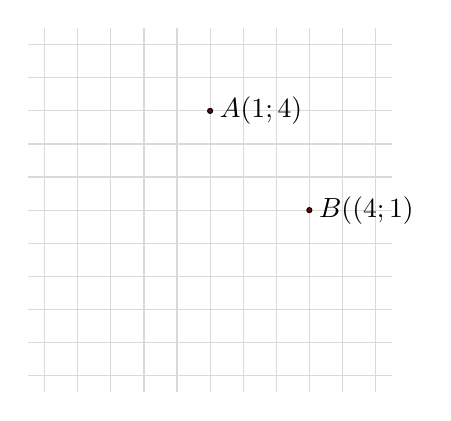
\begin{tikzpicture}[x=7mm, y=7mm, scale=.6]
\draw[step=0.7cm,color=gray!30] (-4.5,-4.5) grid (6.5,6.5);
  \tkzInit[xmin=-4,xmax=6,ymin=-4,ymax=6]
  \begin{scope}[font=\small]
    \tkzAxeX[below = 3pt]
    \tkzAxeY[left = 1pt]
  \end{scope}
  \tkzFct[domain=-5.5:0,thick,color=Maroon]{4/x}
  \tkzFct[domain=-0:5.5,thick,color=Maroon]{4/x}
\tkzFct[domain=-2:6,thick,color=blue]{-x+5};
 \draw[fill=Maroon] (1,4)circle (1.5pt);
\node[right] at (1,4) {$A (1;4)$};
\draw[fill=Maroon] (4,1)circle (1.5pt);
\node[right] at (4,1) {$B ((4;1)$};

\end{tikzpicture}

\end{center}
\end{multicols}
\end{esempio}

\begin{esempio}
Risolvere il seguente sistema 
$\left\{\begin{array}{l}{x+y=1}\\{xy=4}\end{array}\right.$.
\begin{multicols}{2}
L'equazione risolvente è \[ t^2-t+4=0 \] con il discriminante negativo e dunque 
senza soluzioni reali. Il sistema è impossibile.

Possiamo interpretare i risultati ottenuti nel piano cartesiano: la retta di 
equazione $x+y=1$ non interseca l'iperbole equilatera ${xy}=4$.
\begin{center}
% (c) 2013 Claudio Carboncini - claudio.carboncini@gmail.com

\begin{tikzpicture}[x=7mm, y=7mm, scale=.6]
\draw[step=0.7cm,color=gray!30] (-4.5,-4.5) grid (4.5,4.5);
  \tkzInit[xmin=-4.5,xmax=4.5,ymin=-4.5,ymax=4.5]
  \begin{scope}[font=\small]
    \tkzAxeX[orig = false, label options={below = 1pt}]
    \tkzAxeY[orig = true, label options={left = 1pt}]
  \end{scope}
  \tkzFct[domain=-4.5:0,thick,color=Maroon]{1/x}
  \tkzFct[domain=-0:4.5,thick,color=Maroon]{1/x}
\tkzFct[domain=-3:4,thick,color=blue]{-x+1};
\end{tikzpicture}

\end{center}
\end{multicols}
\end{esempio}

\begin{esempio}
Risolvere il seguente sistema 
$\left\{\begin{array}{l}{x+y=2}\\{xy=1}\end{array}\right.$.
\begin{multicols}{2}
L'equazione risolvente è $t^2-2t+1=0$ le cui soluzioni sono: $t_1=t_2=1$.

Il sistema ha due soluzioni coincidenti: \[ 
\left\{\begin{array}{l}{x_1=1}\\{y_1=1}\end{array}\right.\vee 
\left\{\begin{array}{l}{x_2=1}\\{y_2=1}\end{array}\right.. \]

Possiamo interpretare i risultati ottenuti nel piano cartesiano: la retta di 
equazione $x+y=2$ è tangente all'iperbole equilatera $xy=1$ nel punto $(1;1)$.
\begin{center}
% (c) 2013 Claudio Carboncini - claudio.carboncini@gmail.com
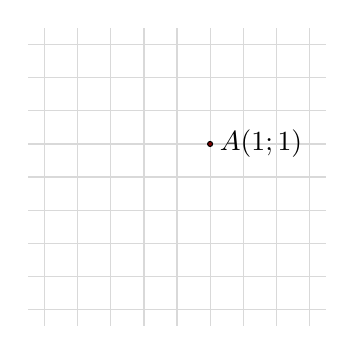
\begin{tikzpicture}[x=7mm, y=7mm, scale=.6]
\draw[step=0.7cm,color=gray!30] (-4.5,-4.5) grid (4.5,4.5);
  \tkzInit[xmin=-4.5,xmax=4.5,ymin=-4.5,ymax=4.5]
  \begin{scope}[font=\small]
    \tkzAxeX[below = 3pt]
    \tkzAxeY[left = 1pt]
  \end{scope}
  \tkzFct[domain=-4.5:0,thick,color=Maroon]{1/x}
  \tkzFct[domain=-0:4.5,thick,color=Maroon]{1/x}
\tkzFct[domain=-3:4,thick,color=blue]{-x+2};
\draw[fill=Maroon] (1,1)circle (1.5pt);
 \node[right] at (1,1) {$A (1;1)$};
\end{tikzpicture}

\end{center}
\end{multicols}
\end{esempio}
\end{exrig}
% \ovalbox{\risolvii \ref{ese:6.14}, \ref{ese:6.15}, \ref{ese:6.16}, 
% \ref{ese:6.17}, \ref{ese:6.18}, \ref{ese:6.19}}

% \subsection{Sistemi simmetrici riconducibili al sistema simmetrico fondamentale}
% In questa categoria rientrano i sistemi simmetrici che, mediante artifici, 
% possono essere trasformati in sistemi simmetrici del tipo precedente.
% 
% \begin{exrig}
% \begin{esempio}
% Risolvere il sistema 
% $\left\{\begin{array}{l}{x+y=a}\\{x^2+y^2+{bx}+{by}=c}\end{array}\right.$.
% 
% È possibile trasformare il sistema in un sistema simmetrico fondamentale.
% 
% Ricordando l'identità $x^2+y^2=(x+y)^2-2{xy}$, il sistema può essere riscritto 
% così: 
% \[ \left\{\begin{array}{l}{x+y=a}\\
% {(x+y)^2-2{xy}+b(x+y)=c}\end{array}\right.
% \Rightarrow \left\{\begin{array}{l}{x+y=a}\\
% {a^2-2{xy}+{ba}=c}\end{array}\right.
% \Rightarrow \left\{\begin{array}{l}{x+y=a}\\
% {{xy}=\frac{a^2+{ab}-c} 2}\end{array}\right..\]
% 
% Posto $a=s$ e $p=\frac{a^2+{ab}-c} 2$ il sistema diventa 
% \[\left\{\begin{array}{l}{x+y=s}\\{{xy}=p}\end{array}\right..\]
% \end{esempio}
% 
% \begin{esempio}
% Risolvere il sistema 
% $\left\{\begin{array}{l}{x+y=7}\\{x^2+y^2=25}\end{array}\right.$
% 
% Ricordando l'identità $x^2+y^2=(x+y)^2-2{xy}$, il sistema può essere riscritto 
% così: 
% \[\left\{\begin{array}{l}{x+y=7}\\
% {(x+y)^2-2{xy}=25}\end{array}\right.
% \Rightarrow \left\{\begin{array}{l}{x+y=7}\\
% {(7)^2-2{xy}=25}\end{array}\right.
% \Rightarrow \left\{\begin{array}{l}{x+y=7}\\
% {-2{xy}=25-49}\end{array}\right.\Rightarrow 
% \left\{\begin{array}{l}{x+y=7}\\{{xy}=12}\end{array}\right..\]
% 
% L'equazione risolvente è $t^2-7t+12=0$ le cui soluzioni sono $t_1=3\vee t_2=4$.
% 
% Le soluzioni del sistema sono: 
% \[\left\{\begin{array}{l}{x_1=3}\\
% {y_1=4}\end{array}\right.\vee \left\{\begin{array}{l}{x_2=4}\\
% {y_2=3}\end{array}\right..\]
% \end{esempio}
% 
% \begin{esempio}
% Risolvere il sistema 
% $\left\{\begin{array}{l}{-3x-3y=-5}\\{2x^2+2y^2=10}\end{array}\right.$
% 
% Dividendo per $-3$ la prima equazione, per $2$ la seconda e ricordando 
% l'identità 
% \[x^2+y^2=(x+y)^2-2{xy}\] 
% si ha: 
% \[ \left\{\begin{array}{l}{x+y=\frac 5 3}\\
% {x^2+y^2=5}\end{array}\right.
% \Rightarrow \left\{\begin{array}{l}{x+y=\frac 5 3}\\
% {(x+y)^2-2{xy}=5}\end{array}\right.
% \Rightarrow \left\{\begin{array}{l}{x+y=\frac 5 3}\\
% {\left(\frac 5 3\right)^2-2{xy}=5}\end{array}\right.
% \Rightarrow \left\{\begin{array}{l}{x+y=\frac 5 3}\\
% {{xy}=-\frac{10} 9}\end{array}\right..\]
% 
% L'equazione risolvente è $t^2-\frac 5 3t-\frac{10} 9=0$ le cui soluzioni sono: 
% $t_1=\frac{5-\sqrt{65}} 6\vee t_2=\frac{5+\sqrt{65}} 6$.
% 
% Le soluzioni del sistema sono le seguenti: 
% \[\left\{\begin{array}{l}{x_1=\frac{5-\sqrt{65}} 6}\\{y_1=\frac{5+\sqrt{65}} 
% 6}\end{array}\right.\vee \left\{\begin{array}{l}{x_2=\frac{5+\sqrt{65}} 
% 6}\\{y_2=\frac{5-\sqrt{65}} 6}\end{array}\right..\]
% \end{esempio}
% \end{exrig}
% \ovalbox{\risolvii \ref{ese:6.20}, \ref{ese:6.21}, \ref{ese:6.22}, 
% \ref{ese:6.23}, \ref{ese:6.24}}
% % 8<
% \subsection{Sistemi non simmetrici riconducibili a sistemi simmetrici}
% Rientrano in questa classe i sistemi che, pur non essendo simmetrici, possono 
% essere trasformati, mediante opportune sostituzioni, in sistemi simmetrici. 
% Naturalmente questi sistemi si possono risolvere anche con la procedura solita 
% di sostituzione per i sistemi di secondo grado.
% 
% \begin{exrig}
% \begin{esempio}
% Risolvere il sistema 
% $\left\{\begin{array}{l}{x-y=8}\\{{xy}=-15}\end{array}\right.$.
% 
% Mediante la sostituzione $y'=-y$ otteniamo 
% $\left\{\begin{array}{l}{x+y'=8}\\{xy'=15}\end{array}\right.$ che è un sistema 
% simmetrico fondamentale.
% 
% L'equazione risolvente è $t^2-8t+15=0$ le cui soluzioni sono $t_1=3\vee t_2=5$, 
% pertanto il sistema ha le soluzioni 
% \[\left\{\begin{array}{l}{x_1=3}\\
% {{y_1}'=5}\end{array}\right.\vee 
% \left\{\begin{array}{l}{x_2=5}\\
% {{y_2}'=3}\end{array}\right..\] 
% Dall'uguaglianza $y'=-y\Rightarrow y=-y'$ otteniamo le soluzioni del sistema 
% dato 
% \[\left\{\begin{array}{l}{x_1=3}\\
% {y_1=-5}\end{array}\right.\vee 
% \left\{\begin{array}{l}{x_2=5}\\
% {y_2=-3}\end{array}\right..\]
% \end{esempio}
% 
% \begin{esempio}
% Risolvere il sistema 
% $\left\{\begin{array}{l}{2x-3y=8}\\{{xy}=2}\end{array}\right.$.
% 
% Mediante la sostituzione $x'=2x$ e $y'=-3y$ da cui $x=\frac{x'} 2$ e 
% $y=-\frac{y'} 3$ otteniamo 
% \[\left\{\begin{array}{l}{x'+y'=8}\\
% {\frac{x'} 2\cdot \left(-\frac{y'} 3\right)=2}\end{array}\right.
% \Rightarrow\left\{\begin{array}{l}{x'+y'=8}\\
% {x'y'=-12}\end{array}\right.\] che è un sistema simmetrico fondamentale.
% 
% Risolviamo il sistema simmetrico 
% $\left\{\begin{array}{l}{x'+y'=8}\\{x'y'=-12}\end{array}\right.$ con la 
% procedura nota. L'equazione risolvente è $t^2-8t-12=0$ le cui soluzioni sono 
% $t_{1,2}=4\pm 2\sqrt 3$ pertanto il sistema ha le soluzioni: 
% \[\left\{\begin{array}{l}{x_1'=4-2\sqrt 7}\\
% {y_1'=4+2\sqrt 7}\end{array}\right.\vee 
% \left\{\begin{array}{l}{x_2'=4+2\sqrt 7}\\
% {y_2'=4-2\sqrt 7}\end{array}\right..\] 
% Dalle sostituzioni $x=\frac{x'} 2$ e $y=-\frac{y'} 3$ otteniamo le soluzioni del 
% sistema iniziale 
% \[\left\{\begin{array}{l}{x_1=\frac{4-2\sqrt 7} 2=2-\sqrt 7}\\
% {y_1=\frac{-4-2\sqrt 7} 3}\end{array}\right.\vee 
% \left\{\begin{array}{l}{x_2=\frac{4+2\sqrt 7} 2=2+\sqrt 7}\\
% {y_2=\frac{-4+2\sqrt 7} 3}\end{array}\right..\]
% \paragraph{Procedura di sostituzione}
% Ricaviamo una delle due incognite dall'equazione di primo grado e sostituiamola 
% nell'altra equazione \[ \left\{\begin{array}{l}{2x-3y=8} 
% \\{{xy}=2}\end{array}\right.\Rightarrow\left\{\begin{array}{l}{y=\frac{2x-8} 
% 3}\\{{xy}=2}\end{array}\right.\Rightarrow \left\{\begin{array}{l}{y=\frac{2x-8} 
% 3}\\{x\left(\frac{2x-8} 3\right)=2}\end{array}\right.\Rightarrow 
% \left\{\begin{array}{l}{y=\frac{2x-8} 3}\\{2x^2-8x-6=0}\end{array}\right.. \]
% 
% Risolviamo l'equazione $2x^2-8x-6=0$ avente come soluzioni $x_1=2-\sqrt 7\vee 
% x_2=2+\sqrt 7$. Applicando la formula ridotta otteniamo: $x_1=2-\sqrt 7\vee 
% x_2=2+\sqrt 7$.
% Sostituiamo i valori trovati e ricaviamo i valori della $y$: \[ 
% \left\{\begin{array}{l}{x_1=2-\sqrt 7}\\{y_1=\frac{-4-2\sqrt 7} 
% 3}\end{array}\right.\vee \left\{\begin{array}{l}{x_2=2+\sqrt 
% 7}\\{y_2=\frac{-4+2\sqrt 7} 3}\end{array}\right.. \]
% \end{esempio}
% \end{exrig}
% \ovalbox{\risolvi \ref{ese:6.25}}
% 
% \subsection{Sistemi simmetrici di grado superiore al secondo}
% Introduciamo le seguenti trasformazioni dette formule di Waring, dal nome del 
% matematico che le ha formulate per primo. Con tali formule, si possono 
% trasformare le potenze di un binomio in relazioni tra somme e prodotti delle due 
% variabili che lo compongono. Indicate come $s$ somma delle variabili e $p$ il 
% loro prodotto queste sono le prime formule fino alla potenza quinta.
% \begin{itemize*}
% \item $ a^2+b^2=(a+b)^2-2{ab}=s^2-2p $
% \item $ a^3+b^3=(a+b)^3-3a^2b-3ab^2=(a+b)^3-3{ab}(a+b)=s^3-3{ps} $
% \item $ a^4+b^4=s^4-4{ps}^2+2p^2 $
% \item $ a^5+b^5=s^5-5{ps}^3+5p^2s $.
% \end{itemize*}
% 
% \begin{exrig}
% \begin{esempio}
% Risolvere il sistema 
% $\left\{\begin{array}{l}{x+y=1}\\{x^3+y^3-2{xy}=3}\end{array}\right.$.
% 
% Applicando l'identità $x^3+y^3=(x+y)^3-3{xy}(x+y)$, il sistema può essere 
% riscritto così: \[ 
% \left\{\begin{array}{l}{x+y=1}\\{(x+y)^3-3{xy}(x+y)-2{xy}=3}\end{array}
% \right.\Rightarrow 
% \left\{\begin{array}{l}{x+y=1}\\{1-5{xy}=3}\end{array}\right.\Rightarrow 
% \left\{\begin{array}{l}{x+y=1}\\{{xy}=-\frac 2 5}\end{array}\right..\]
% 
% Da cui l'equazione risolvente $t^2-t-\frac 2 5=0\Rightarrow 5t^2-5t-2=0$ con 
% $t_1=\frac{5-\sqrt{65}}{10}$ e $t_2=\frac{5+\sqrt{65}}{10}$.
% Le soluzioni del sistema sono: 
% $\left(\frac{5-\sqrt{65}}{10};\frac{5+\sqrt{65}}{10}\right),\left(\frac{5+\sqrt{
% 65}}{10};\frac{5-\sqrt{65}}{10}\right)$.
% \end{esempio}
% 
% \begin{esempio}
% Risolvere il sistema $\left\{\begin{array}{l}{x+y=-1}\\{x^4+y^4=\frac 7 
% 2}\end{array}\right.$.
% 
% Ricordando l'identità $x^4+y^4=(x+y)^4-4{xy}(x+y)^2+2x^2y^2$, il sistema può 
% essere riscritto così: 
% \[\left\{\begin{array}{l}{x+y=-1}\\{(x+y)^4-4{xy}(x+y)^2+2x^2y^2=\frac 7 
% 2}\end{array}\right. \Rightarrow 
% \left\{\begin{array}{l}{x+y=-1}\\{2x^2y^2-4{xy}-\frac 5 
% 2=0}\end{array}\right..\]
% 
% Introduciamo l'incognita ausiliaria $u=xy$. L'equazione $2x^2y^2-4{xy}-\frac 5 
% 2=0$ diventa $2u^2-4u-\frac 5 2=0$ che ha come soluzioni $u_1=-\frac 1 2\vee 
% u_2=\frac 5 2\Rightarrow {xy}=-\frac 1 2\vee {xy}=\frac 5 2$.
% 
% Il sistema assegnato è equivalente a due insiemi 
% \[\left\{\begin{array}{l}{x+y=-1}\\{{xy}=-\frac 1 2}\end{array}\right.\vee 
% \left\{\begin{array}{l}{x+y=-1}\\{{xy}=\frac 5 2}\end{array}\right.\] 
% e dunque il suo insieme soluzione $S$ si ottiene dall'unione dell'insieme 
% soluzione dei due 
% sistemi~$S=S_1\cup S_2$.
% 
% Il primo sistema 
% \[\left\{\begin{array}{l}{x+y=-1}\\{{xy}=-\frac 1 2}\end{array}\right.\] 
% ha equazione risolvente $t^2+t-\frac 1 2=0$ con 
% \[t_1=\frac{-1-\sqrt 3} 2\text{ e }t_2=\frac{-1+\sqrt 3} 2.\] 
% Il sistema ha soluzioni 
% \[\left(\frac{-1-\sqrt 3} 2;\frac{-1+\sqrt 3} 2\right),\left(\frac{-1+\sqrt 3} 
% 2;\frac{-1-\sqrt 3} 2\right)\] e quindi \[S_1=\left\{\left(\frac{-1-\sqrt 3} 
% 2;\frac{-1+\sqrt 3} 2\right),\left(\frac{-1+\sqrt 3} 2;\frac{-1-\sqrt 3} 
% 2\right)\right\}.\]
% 
% Il secondo sistema $\left\{\begin{array}{l}{x+y=-1}\\{{xy}=\frac 5 
% 2}\end{array}\right.$ ha equazione risolvente $t^2+t+\frac 5 2=0$, che ha 
% $\Delta <0$, l'insieme soluzione è vuoto. Anche il sistema non ha soluzioni 
% reali, quindi $S_2=\emptyset $. L'insieme soluzione del sistema assegnato 
% $\left\{\begin{array}{l}{x+y=-1}\\{x^4+y^4=\frac 7 2}\end{array}\right.$ è 
% $S=S_1\cup \emptyset =S_1$.
% \end{esempio}
% \end{exrig}
% \ovalbox{\risolvii \ref{ese:6.26}, \ref{ese:6.27}, \ref{ese:6.28}, 
% \ref{ese:6.29}, \ref{ese:6.30}, \ref{ese:6.31}, \ref{ese:6.32}, \ref{ese:6.33}, 
% \ref{ese:6.34}, \ref{ese:6.35}}
% 
% \section{Sistemi omogenei di quarto grado}
% Un sistema si dice omogeneo se le equazioni, con l'eccezione dei termini noti, 
% hanno tutti i termini con lo stesso grado. I sistemi omogenei di quarto grado 
% sono quindi nella forma:
% \begin{equation*}
% \left\{\begin{array}{l}{{ax}^2+{bxy}+{cy}^2=d}\\{a'x^2+b'{xy}+c'y^2=d'}\end{
% array}\right..
% \end{equation*}
% \paragraph{Primo caso} $d=0 \wedge d'=0$.
% 
% Il sistema si presenta nella forma 
% $\left\{\begin{array}{l}{{ax}^2+{bxy}+{cy}^2=0}\\{a'x^2+b'{xy}+c'y^2=0}\end{
% array}\right.$. Un sistema di questo tipo ha sempre almeno la soluzione nulla $ 
% (0; 0) $.
% 
% Per trovare le soluzioni del sistema poniamo $y={tx}$ sostituendo abbiamo: \[ 
% \left\{\begin{array}{l}{{ax}^2+{btx}^2+{ct}^2x^2=0}\\{a'x^2+b'{tx}^2+c't^2x^2=0}
% \end{array}\right. \text{ da cui } 
% \left\{\begin{array}{l}{x^2(a+{bt}+{ct}^2)=0}\\{x^2(a'+b't+c't^2)=0}\end{array}
% \right.. \]
% 
% Supponendo $x\neq 0$ e che quindi che può assumere tutti i valori $k\in \insR_0$ 
% possiamo dividere le due equazioni per $x^2$, otteniamo così due equazioni 
% nell'incognita $t$ che possiamo risolvere. Se le due equazioni ammettono qualche 
% soluzione comune allora il sistema ammette infinite soluzioni. Le soluzioni sono 
% del tipo $x=k$ e $y={kt}$, dove $t$ è la soluzione comune di cui si è detto 
% prima.
% 
% \begin{exrig}
% \begin{esempio}
% Risolvere il seguente sistema $\left\{\begin{array}{l}x^2-3{xy}+2y^2=0 
% \\-x^2+5{xy}-6y^2=0 \end{array}\right.$.
% 
% Applichiamo la sostituzione $y={tx}$, il sistema diventa 
% $\left\{\begin{array}{l}x^2-3{tx}^2+2t^2x^2=0 \\-x^2+5{tx}^2-6t^2x^2=0 
% \end{array}\right.$.
% 
% Dividendo per $x^2$ otteniamo $\left\{\begin{array}{l}1-3t+2t^2=0 \\1-5t+6t^2=0 
% \end{array}\right.$.
% 
% La prima equazione è risolta per $t_1=1\vee t_2=\frac 1 2$, mentre la seconda 
% equazione è risolta per $t_3=\frac 1 2\vee t_4=\frac 1 3$. Le due equazioni 
% hanno una radice in comune $t=\frac 1 2$.
% 
% Pertanto oltre alla soluzione $(0;0)$ il sistema ammette infinite soluzioni che 
% possono essere scritte nella forma $\left\{\begin{array}{l}x=k \\y=\frac 1 2k 
% \end{array}\right.$.
% \end{esempio}
% \end{exrig}
% 
% \paragraph{Secondo caso}$d=0 \wedge d'\neq 0$.
% 
% Il sistema si presenta nella forma 
% $\left\{\begin{array}{l}{{ax}^2+{bxy}+{cy}^2=0}\\{a'x^2+b'{xy}+c'y^2=d'}\end{
% array}\right.$.
% 
% Ponendo $y={tx}$ si ha 
% $\left\{\begin{array}{l}{{ax}^2+{btx}^2+{ct}^2x^2=0}\\{a'x^2+b'{tx}
% ^2+c't^2x^2=d'}\end{array}\right.$.
% 
% Dividendo per $x^2$ la prima equazione si ha 
% $\left\{\begin{array}{l}{a+{bt}+{ct}^2=0}\\{x^2(a'+b't+c't^2)=d'}\end{array}
% \right.$.
% 
% Si risolve la prima equazione nell'incognita $t$ si sostituiscono i valori 
% trovati nella seconda equazione e si ricavano i valori di $x$ e di seguito i 
% valori di $y$ con $y={tx}$.
% \newpage
% \begin{exrig}
% \begin{esempio}
% Risolvere il sistema $\left\{\begin{array}{l}x^2-{xy}-6y^2=0 
% \\-x^2+2{xy}-3y^2=-6 \end{array}\right.$.
% 
% Sostituendo $y={tx}$ il sistema diventa 
% \[\left\{\begin{array}{l}1-t-6t^2=0 \\x^2(-1+2t-3t^2)=-6 \end{array}\right..\]
% 
% La prima equazione ha per soluzioni $t_1=\frac 1 3$ e $t_2=-\frac 1 2$.
% 
% Sostituendo $t=\frac 1 3$ nella seconda equazione si ha $x_{1,2}=\pm 3$ e 
% sapendo che $y={tx}$ si ottengono le coppie 
% \[\left\{\begin{array}{l}x_1=3\\y_1=1\end{array}\right.\vee\left\{\begin{array}{
% l}x_2=-3\\y_2=-1\end{array}\right..\]
% 
% Sostituendo $t=-\frac 1 2$ si ha $x_3=-\frac{2\sqrt 6}{11}\vee x_4=\frac{2\sqrt 
% 6}{11}$ e sapendo che $y={tx}$ si ottengono le coppie 
% \[\left\{\begin{array}{l}x_3=-\frac{2\sqrt 6}{11}\\y_3=\frac{\sqrt 
% 6}{11}\end{array}\right.\vee\left\{\begin{array}{l}x_4=-2\frac{\sqrt 
% 6}{11}\\y_4=-\frac{\sqrt 6}{11}\end{array}\right..\]
% 
% L'insieme soluzione del sistema è 
% \[\IS=\left\{(x_1;y_1),(x_2;y_2),(x_3;y_3),(x_4;y_4)\right\}.\]
% \end{esempio}
% \end{exrig}
% 
% \paragraph{Terzo caso} $d\neq 0 \wedge d'\neq 0$.
% 
% Il sistema si presenta nella forma 
% $\left\{\begin{array}{l}{{ax}^2+{bxy}+{cy}^2=d}\\{a'x^2+b'{xy}+c'y^2=d'}\end{
% array}\right.$.
% 
% Ponendo $y=tx$ si ha 
% \[\left\{\begin{array}{l}{x^2(a+{bt}+{ct}^2)=d}\\{x^2(a'+b't+c't^2)=d'}\end{
% array}\right..\]
% Dividendo membro a membro le due equazioni, sotto la condizione $x\neq 0\wedge 
% a'+b't+c't^2\neq 0$ otteniamo 
% \begin{align*}
% &\frac{a+{bt}+{ct}^2}{a'+b't+c't^2}=\frac d{d'}\\
% \Rightarrow & d'(a+{bt}+{ct}^2)=d(a'+b't+c't^2)\\
% \Rightarrow & ({cd}'-c'd)t^2+({bd}'-b'd)t+{ad}'-a'd=0 
% \end{align*}
% che è una equazione di secondo grado nell'incognita $t$.
% 
% Se l'equazione ha come soluzioni $t_1$ e $t_2$ dobbiamo poi risolvere i sistemi 
% \[ \left\{\begin{array}{l}y=t_1x \\a'x^2+b'{xy}+c'y^2=d' 
% \end{array}\right.\vee\left\{\begin{array}{l}y=t_2x \\a'x^2+b'{xy}+c'y^2=d' 
% \end{array}\right.. \]
% \newpage
% \begin{exrig}
% \begin{esempio}
% Risolvere il sistema $\left\{\begin{array}{l}x^2+3{xy}-y^2=-68 
% \\-2x^2+{xy}+3y^2=88 \end{array}\right.$.
% 
% Sostituendo $y={tx}$ il sistema diventa 
% $\left\{\begin{array}{l}x^2(1+3t-t^2)=-68 \\x^2(-2+t+3t^2)=88 
% \end{array}\right.$.
% 
% Dividendo membro a membro con la condizione $x\neq 0\wedge 3t^2+t-2\neq 0$ cioè 
% $x\neq 0$, $t\neq -1$ e $t\neq \frac 2 3$ si ha 
% $\frac{1+3t-t^2}{-2+t+3t^2}=-\frac{68}{88}$, da cui l'equazione $29t^2+83t-12=0$ 
% con soluzioni $t_1=\frac 4{29}\vee t_2=-3$.
% 
% A questo punto dobbiamo risolvere i due sistemi:\[ 
% \left\{\begin{array}{l}y=\frac 4{29}x \\-2x^2+{xy}+3y^2=88 
% \end{array}\right.\vee\left\{\begin{array}{l}y=-3x \\-2x^2+{xy}+3y^2=88 
% \end{array}\right.. \]
% 
% Il primo sistema è impossibile, il secondo ha soluzioni 
% \[\left\{\begin{array}{l}x_1=-2\\y_1=6\end{array}\right.\vee\left\{\begin{array}
% {l}x_2=2\\y_2=-6\end{array}\right..\] 
% L'insieme soluzione del sistema è $\IS=\{(-2;6),(2;-6)\}$.
% \end{esempio}
% \end{exrig}
% \ovalbox{\risolvii \ref{ese:6.36}, \ref{ese:6.37}, \ref{ese:6.38}, 
% \ref{ese:6.39}, \ref{ese:6.40}, \ref{ese:6.41}, \ref{ese:6.42}, \ref{ese:6.43}, 
% \ref{ese:6.44}, \ref{ese:6.45}, \ref{ese:6.46}, \ref{ese:6.47}, \ref{ese:6.48}.}
% 
% \section{Problemi che si risolvono con sistemi di grado superiore al primo}
% Riprendiamo un problema già discusso. Considerare più variabili ci permette di 
% facilitare il processo di traduzione in linguaggio matematico.
% 
% \begin{problema}
% Il trapezio isoscele ${ABCD}$ è inscritto in una semicirconferenza di diametro 
% ${AB}$ di misura $25\unit{cm}$ determinare le misure dei lati del trapezio 
% sapendo che il perimetro è $62\unit{cm}$.
% \end{problema}
% \begin{multicols}{2}
% \emph{Dati}: $\begin{array}{l}\overline{AB}=25;2p=62;\\{AB}\parallel 
% {DC};{AD}\equiv {CB}\end{array}$.
% 
% \emph{Obiettivo}: $\overline{CB}$ $\overline{DC}$.
% 
% \emph{Dati impliciti}: $\begin{array}{l}
% \overline{{KO}}=\overline{{CH}}; \overline{{CO}}=\frac{25} 2;\\ 
% \overline{{KC}}=\frac{\overline{{DC}}} 2; \overline{{HB}}=\frac{25-y} 2;\\ 
% \widehat {{CKO}}=90\grado; \widehat {{CHB}}=90\grado.\end{array}$
% 
% \emph{Incognite}: $\overline{{CB}}=x$ $\overline{{DC}}=y$.
% 
% \emph{Vincoli: } $\left\{\begin{array}{l}0<x<\frac{25} 2\sqrt 2\\0<y<25 
% \end{array}\right.$.
% \begin{center}
% % (c) 2013 Claudio Carboncini - claudio.carboncini@gmail.com
\begin{tikzpicture}[x=10mm,y=10mm,font=\small]
  \coordinate(a) at (-2.5,0);
  \coordinate(d) at (130:2.5);
  \coordinate(e) at (90:2.5);
  \coordinate(c) at (50:2.5);
  \coordinate(b) at (2.5,0);
  \coordinate(o) at (0,0);
  \coordinate (h) at ($(a)!(c)!(b)$);%trova le coordinate della proiezione di c su a--b
  \coordinate (k) at ($(d)!(e)!(c)$);%trova le coordinate della proiezione di e su d--c
  \fill[color=gray!20](o)--(k)--(c);
  \fill[color=gray!20](h)--(b)--(c);
  \draw (-2.5,0) arc (180:0:2.5) -- cycle;% semicirconferenza e diametro
  \draw (a) -- (d) -- (c) -- (b);%disegna il trapezio
  \draw [dashdotted] (e) -- (0,0);%da E a O
  \draw [dotted] (c) -- (h);% c--h
 \draw [dotted] (o) -- (c);% o--c
  \node [label={[name=label node]below left:$A$}] at (a) {};
  \node [label={[name=label node]below right:$B$}] at (b) {};
  \node [label={[name=label node]above right:$C$}] at (c) {};
  \node [label={[name=label node]above left:$D$}] at (d) {};
  \node [label={[name=label node]above:$E$}] at (e) {};
  \node [label={[name=label node]below:$H$}] at (h) {};
  \node [label={[name=label node]below left:$K$}] at (k) {};
  \node [label={[name=label node]below:$O$}] at (o) {};
  \node[] at (2.1,-.3) {$\frac{25-y}2$};
  \node[] at (25:2.4) {$x$};
  \node[] at (70:2.25) {$\frac y 2$};
  \node[] at (45:1.25) {$\frac {25} 2$};
  \filldraw[fill=black, draw=black]  (a) circle (1pt);
  \filldraw[fill=black, draw=black]  (b) circle (1pt);
  \filldraw[fill=black, draw=black]  (c) circle (1pt);
  \filldraw[fill=black, draw=black]  (d) circle (1pt);
  \filldraw[fill=black, draw=black]  (h) circle (1pt);
  \filldraw[fill=black, draw=black]  (e) circle (1pt);
  \filldraw[fill=black, draw=black]  (k) circle (1pt);
  \filldraw[fill=black, draw=black]  (o) circle (1pt);

\end{tikzpicture}

% \end{center}
% \end{multicols}
% 
% \emph{Relazioni tra dati e incognite}:
% $\left\{\begin{array}{l}{y+2x+25=62}\\{\left(\frac{25} 2\right)^2-\left(\frac y 
% 2\right)^2=x^2-\left(\frac{25-y} 2\right)^2}\end{array}\right. \Rightarrow 
% \left\{\begin{array}{l}{y=-2x+37}\\{x^2-25x+150=0}\end{array}\right.. $
% 
% \emph{Soluzioni: } 
% $\left\{\begin{array}{l}{x_1=15}\\{y_1=7}\end{array}\right.\vee 
% \left\{\begin{array}{l}{x_2=10}\\{y_2=17}\end{array}\right.$.
% 
% \emph{Verifica: }Entrambe le soluzioni sono accettabili.
% 
% La risoluzione del problema si basa sulla equazione di primo grado $y+2x+25=62$ 
% che definisce il perimetro, sulla congruenza dei segmenti $\overline{{KO}}$ e 
% $\overline{{CH}}$ facilmente dimostrabile in quanto stessa distanza tra due 
% rette parallele, l'applicazione del teorema di Pitagora ai triangoli ${CKB}$ e 
% ${CHB}$ rettangoli per costruzione. Naturalmente tutte le informazioni ausiliare 
% vanno dimostrate, ma data la loro facilità le lasciamo al lettore.
% 
% Importante è impostare le condizioni sulle incognite che devono essere maggiori 
% di $0$ ma anche $x<\frac{25} 2\sqrt 2$ perché il trapezio non diventi un 
% triangolo e $y<25$ perché la base minore sia realmente minore. L'ultimo passo 
% consiste nella verifica delle soluzioni, che nel nostro caso sono entrambe 
% accettabili. Si hanno dunque due trapezi inscritti in quella semicirconferenza 
% che avranno il perimetro di 62 cm.
% 
% \begin{problema}
% L'azienda Profit intende fare una ristrutturazione riducendo il numero degli 
% operai. Oggi spende per gli operai (tutti con lo stesso stipendio) 800 € al 
% giorno. Se si licenziassero 5 dipendenti e si riducesse lo stipendio di 2 € al 
% giorno si avrebbe un risparmio giornaliero di 200 €. Quanti sono gli operai 
% attualmente occupati nell'azienda?
% \end{problema}
% 
% \emph{Dati}:$ \begin{array}{l}
% \text{spesa per salari al giorno}= 800\unit{\text{€}};\\
% \text{riduzione salario giornaliero}= 2\unit{\text{€}};\\
% \text{riduzione numero operai}= 5\text{ unità};\\
% \text{risparmio dopo il licenziamento e la riduzione di stipendio}= 
% 200\unit{\text{€}}.
% \end{array}$
% 
% \emph{Obiettivo}: numero operai occupati prima della ristrutturazione
% 
% \emph{Incognite}:$ \begin{array}{l}
% x = \text{numero operai prima della ristrutturazione};\\
% y = \text{salario percepito da ogni operaio prima della ristrutturazione}.
% \end{array}$
% 
% \emph{Vincoli}: $\left\{\begin{array}{l}x\in \insN\\y\in 
% \insR^+\end{array}\right.$
% 
% \emph{Altre Informazioni}: $ \begin{array}{l}
% \text{Numero operai dopo la ristrutturazione} = x-5;\\
% \text{salario dopo la ristrutturazione} =y-2;\\
% \text{spesa per stipendi dopo la ristrutturazione} 
% =800-200=600\unit{\text{€}}.\end{array}$
% 
% \emph{Relazioni tra dati e incognite}:
% \begin{equation*}
% \left\{\begin{array}{l}{{xy}=800}\\{(x-5)(y-2)=600}\end{array}\right.\Rightarrow 
% \left\{\begin{array}{l}{{xy}=800}\\{{xy}-2x-5y+10=600}\end{array}
% \right.\Rightarrow 
% \left\{\begin{array}{l}{{xy}=800}\\{2x+5y=210}\end{array}\right.
% \end{equation*}
% 
% \emph{Soluzioni}: 
% $\left\{\begin{array}{l}{x_1=25}\\{y_1=32}\end{array}\right.\vee 
% \left\{\begin{array}{l}{x_2=80}\\{y_2=10}\end{array}\right.$
% 
% \emph{Verifica}: Entrambe le soluzioni sono accettabili.
% 
% Naturalmente c'è una grande differenza tra percepire $32\unit{\text{€/giorno}}$ 
% di salario o $ 10\unit{\text{€/giorno}} $, come avere impiegati $ 25 $ o $ 80 $ 
% operai. Il problema va meglio definito. Basterebbe per questo un vincolo che ci 
% dice qual è la paga minima giornaliera di un operaio.
% 
% \begin{problema}
% Un numero $k\in \insN$ è composto da tre cifre. Il prodotto delle tre cifre è 
% $42$. Se si scambia la cifra delle decine con quella delle centinaia si ottiene 
% un numero che supera $k$ di $360$. Se si scambia la cifra della unità con quella 
% delle centinaia si ottiene un numero minore di $99$ rispetto al numero $k$. 
% Trovare $k$.
% \end{problema}
% 
% \emph{Dati}: $\begin{array}{l}
% \text{il numero } k \text{ è composto da tre cifre};\\
% \text{prodotto delle tre cifre } = 42;\\
% \text{scambiando la cifra delle decine con quella delle centinaia otteniamo 
% }l=k+360; \\
% \text{scambiando la cifra delle unità con quella delle centinaia otteniamo } 
% m=k-99.\\
% \end{array}$
% 
% \emph{Obiettivo}: trovare il numero $k$.
% 
% \emph{Incognite}: $\begin{array}{l}
% x =\text{ cifra che rappresenta il numero delle centinaia;}\\
% y=\text{ cifra che rappresenta il numero delle decine;}\\
% z=\text{ cifra che rappresenta il numero delle unità.}
% \end{array}$
% 
% \emph{Vincoli}: $\left\{\begin{array}{l}x\in \{1,2,3,4,5,6,7,8,9\} \\y,z\in 
% \{0,1,2,3,4,5,6,7,8,9\}\end{array}\right.$.
% 
% \emph{Altre Informazioni}: $\begin{array}{l}
% k=100x+10y+z;\\
% l=100y+10x+z;\\
% m=100z+10y+x.
% \end{array}$
% 
% \emph{Relazioni tra dati e incognite}: \[ \left\{\begin{array}{l}x\cdot y\cdot 
% z=42 \\100y+10x+z=100x+10y+z+360\\100z+10y+x=100x+10y+z-99 
% \end{array}\right.\Rightarrow \left\{\begin{array}{l}x\cdot y\cdot z=42 
% \\x-y=-4\\x-z=1\end{array}\right.. \]
% 
% \emph{Soluzioni}: 
% $\left\{\begin{array}{l}x_1=3\\y_1=7\\z_1=2\end{array}\right.$.
% 
% \emph{Verifica}: La soluzione soddisfa le condizioni il numero cercato è $372$.
% 
% \vspazio
% \ovalbox{\risolvii \ref{ese:6.49}, \ref{ese:6.50}, \ref{ese:6.51}, 
%          \ref{ese:6.52}, \ref{ese:6.53}, \ref{ese:6.54}, \ref{ese:6.55}, 
%          \ref{ese:6.56}, \ref{ese:6.47}, \ref{ese:6.58}, \ref{ese:6.59}, 
%          \ref{ese:6.60}, \ref{ese:6.61}}
% 
% \vspazio
% \ovalbox{\ref{ese:6.62}, \ref{ese:6.63}, \ref{ese:6.64}, \ref{ese:6.65}, 
%          \ref{ese:6.66}, \ref{ese:6.67}, \ref{ese:6.68}, \ref{ese:6.69}, 
%          \ref{ese:6.70}, \ref{ese:6.71}}
% % >8